\documentclass[11pt,a4paper]{article}
\usepackage[T1]{fontenc}
\usepackage[utf8]{inputenc}
\usepackage{lmodern,microtype}
\usepackage[margin=25mm]{geometry}
\usepackage{amsmath,amssymb,amsthm,mathtools}
\usepackage{booktabs,array,tabularx,enumitem}
\usepackage{xcolor}
\usepackage{tikz}
\usetikzlibrary{arrows.meta,positioning,shapes.geometric,fit,calc}
\usepackage[colorlinks=true,linkcolor=blue!55!black,citecolor=teal!70!black,urlcolor=blue!55!black]{hyperref}
\hypersetup{pdftitle={Exact Gaussian range laws for structured sketches}}

\newtheorem{theorem}{Theorem}[section]
\newtheorem{lemma}[theorem]{Lemma}
\newtheorem{proposition}[theorem]{Proposition}
\newtheorem{corollary}[theorem]{Corollary}
\newtheorem{mainthm}{Theorem}
\renewcommand{\themainthm}{\Alph{mainthm}}
\theoremstyle{definition}
\newtheorem{definition}[theorem]{Definition}
\newtheorem{example}[theorem]{Example}
\theoremstyle{remark}
\newtheorem{remark}[theorem]{Remark}
\numberwithin{equation}{section}

\newcommand{\E}{\mathbb E}
\newcommand{\Prob}{\mathbb P}
\newcommand{\R}{\mathbb R}
\newcommand{\C}{\mathbb C}
\newcommand{\T}{{\mathsf T}}
\newcommand{\tr}{\operatorname{tr}}
\newcommand{\rank}{\operatorname{rank}}
\newcommand{\range}{\operatorname{range}}
\newcommand{\diag}{\operatorname{diag}}
\newcommand{\sym}{\operatorname{sym}}
\newcommand{\Var}{\operatorname{Var}}
\newcommand{\Gr}{\operatorname{Gr}}
\newcommand{\RP}{\mathbb{RP}}
\newcommand{\norm}[1]{\lVert#1\rVert}
\newcommand{\eps}{\varepsilon}
\newcommand{\kapG}{\kappa_{\mathrm G}}
\newcommand{\F}{\mathrm F}
\newcommand{\GN}{\mathrm{GN}}

\setlength{\emergencystretch}{3em}
\setlist{itemsep=2pt,topsep=4pt}

\title{Exact Gaussian range laws for structured sketches}
\author{}
\date{29 September 2026}

% Shared manuscript typography. Keep this file beside the manuscript folders.
\usepackage{needspace}
\usepackage{etoolbox}
\linespread{1.08}
\setlength{\parskip}{0.38em plus 0.08em minus 0.05em}
\setlength{\parindent}{1.25em}
\setlength{\emergencystretch}{2em}
\setlist{itemsep=4pt,topsep=6pt,parsep=2pt}
\renewcommand{\arraystretch}{1.16}
\setlength{\tabcolsep}{6pt}
\AtBeginDocument{%
  \setlength{\abovedisplayskip}{10pt plus 2pt minus 2pt}%
  \setlength{\belowdisplayskip}{10pt plus 2pt minus 2pt}%
  \setlength{\abovedisplayshortskip}{5pt plus 2pt}%
  \setlength{\belowdisplayshortskip}{8pt plus 2pt minus 2pt}%
}
\makeatletter
\def\th@plain{%
  \thm@preskip=10pt plus 2pt minus 2pt
  \thm@postskip=10pt plus 2pt minus 2pt
  \itshape
}
\def\th@definition{%
  \thm@preskip=10pt plus 2pt minus 2pt
  \thm@postskip=10pt plus 2pt minus 2pt
  \normalfont
}
\def\th@remark{%
  \thm@headfont{\itshape}%
  \thm@preskip=9pt plus 2pt minus 2pt
  \thm@postskip=9pt plus 2pt minus 2pt
  \normalfont
}
\makeatother
\AtBeginEnvironment{proof}{\Needspace{4\baselineskip}}
\widowpenalty=10000
\clubpenalty=10000
\displaywidowpenalty=10000
\raggedbottom

\begin{document}
\maketitle
\begin{abstract}
When does a structured sketch produce exactly the same approximation as a
dense Gaussian sketch \emph{in distribution}? For a fixed input support and
independent columns, we prove a necessary and sufficient condition: each
projected column is nonzero and its line is uniform on projective space.
This identifies exact Gaussian laws for rangefinders, PSD Nystr\"om, and
powered or Krylov ranges. Conditional scalar Gaussianity supplies explicit
Khatri--Rao and tensor-train examples. On these supports, the classical
Nystr\"om coefficient $r/(k-r-1)$ holds without a tensor-dependent penalty.
The restriction is substantial: product probes require support dimension at
most $1+\sum_j(n_j-1)$, and the conditional product class reduces to an
$n_1\times n_1$ matrix. We exploit that reduction to transfer Gaussian
generalized Nystr\"om and trace estimators to legal product queries.
Counterexamples show why the full support hypothesis, left-side calibration,
and the distinction between range and embedding laws are essential.
\end{abstract}

\tableofcontents

\section{Introduction}\label{sec:intro}

Let $A\in\R^{N_L\times N}$ be a fixed matrix and $\Omega\in\R^{N\times k}$ a
random test matrix. A rangefinder forms $Y=A\Omega$ and approximates $A$ by
$P_YA$, where $P_Y$ is the orthogonal projector onto $\range Y$.
Multiplying one column of $Y$ by a nonzero scalar does not change $P_Y$.
Neither does multiplying a column of $\Omega$ by a nonzero scalar. This
elementary fact has a sharp consequence for structured sketches: whatever
random column scales a structured probe carries, they are invisible to every
output that depends only on the spanned subspace.

The question we answer is: \emph{exactly when does a structured sketch give
the same output law as a dense Gaussian sketch, for range-determined
outputs?} The answer (Theorem~\ref{mthm:iff}) is a statement about one
column: its projection onto the relevant support must have a uniformly
distributed line. The answer is exact, not asymptotic.\footnote{The phrase
``Gaussian equivalence'' is also used for asymptotic universality of random
feature models. The statements here are exact and finite-dimensional.}

The practical interest comes from tensor-structured probes such as
Khatri--Rao products $g\otimes h$ and tensor trains. These have cheap
matrix--vector products in tensor formats, but their projected coordinates
share random scales, and their sketch Gram matrices are not Wishart. On the
class identified here, those scales cancel from the range, and the sharp
Gaussian constants hold verbatim. For example, common-Schmidt Khatri--Rao
Nystr\"om has expected trace error at most $(1+r/(k-r-1))$ times optimal
(Corollary~\ref{cor:kr}). This is the classical Gaussian coefficient. Its
appearance here follows from equality of output laws, rather than from an
improved embedding estimate.

We are equally explicit about what the class is. A dimension count shows
that a product probe can meet the criterion only on supports of dimension at
most $\sum_j(n_j-1)+1$ (Theorem~\ref{mthm:ceiling}). For the conditionally
Gaussian product class the rank is at most $n_1$, and the whole problem
reduces exactly to an $n_1\times n_1$ matrix reachable by one product query
per matrix--vector product (Theorem~\ref{mthm:reduction}). The class-specific
results should therefore be read as exact identifications and as clean
product-query transfers of Gaussian algorithms. Their algorithmic content is
largest when $n_1$ is large compared with the target rank or accuracy budget.

\subsection{Prior work and the contribution of this paper}

Gaussian rangefinding and its pseudoinverse analysis are classical
\cite{HMT}. The PSD approximation and truncation bounds used below come from
Tropp, Yurtsever, Udell and Cevher \cite{TYUCpsd}; the corresponding two-sketch
reconstruction is developed in \cite{TYUCgeneral,Nak}. Hutch++ and
Nystr\"om++ already establish the $O(\eps^{-1})$ trace-estimation principle
\cite{Hutchpp,Nyspp}. We include proofs of the Gaussian estimates needed here
to isolate exactly what is transferred to product queries.

For structured sketches, Bujanovi\'c, Grubi\v{s}i\'c, Kressner and Lam
\cite{BGKL}, Saibaba, Verma and Ballard \cite{SVB}, and Beretta and Musco
\cite{BM} study Khatri--Rao embeddings or approximation guarantees on general
fixed subspaces. Cama\~no, Epperly, Meyer and Tropp \cite{CEMT} organize
structured approximation around oblivious subspace injections. Those results
address broad input classes. The condition studied here is stronger and
holds on a restricted full support: it identifies the entire finite-sample
output law, including its tails, rather than only an error guarantee.

The contribution is the use of projective uniformity as a complete criterion
for these output laws, together with concrete support certificates, a rank
obstruction, and an exact product-query reduction. The rotation invariance,
inverse-Wishart moments, Hurwitz identities \cite{LMO}, and Gaussian
algorithms underlying the argument are established facts. The new
class-specific consequences are one-response calibration and the calibrated
or frozen-environment implementations. The numerical evidence supports these
identities; it does not establish priority or a general-input improvement.

\subsection{Setting and notation}

Throughout, $\norm\cdot$ is the Euclidean norm on vectors, $\norm\cdot_\F$ the
Frobenius norm, and $M^\dagger$ the Moore--Penrose pseudoinverse. For a PSD
matrix $A$ with eigenvalues $\lambda_1\ge\lambda_2\ge\cdots$ we write
$\tau_r(A)=\sum_{j>r}\lambda_j(A)$; for a rectangular matrix
$\tau^{(2)}_r(A)=\sum_{j>r}\sigma_j(A)^2$. The Grassmannian of $j$-dimensional
subspaces of $\R^R$ is $\Gr(j,R)$, and $\RP^{R-1}=\Gr(1,R)$. We write
$\mathcal G_R=\bigsqcup_{j=0}^R\Gr(j,R)$ for the space of all subspaces, with
its Borel structure. For a nonzero vector $x$, $[x]$ is the line it spans.

A \emph{probe} is a random vector $\omega\in\R^N$. A \emph{sketch} of size $k$
is $\Omega=[\omega_1\ \cdots\ \omega_k]$. Unless explicitly stated
otherwise, the columns are independent copies of $\omega$. When a probe is
generated with auxiliary randomness (an \emph{environment}), the pairs
(probe, environment) are independent across columns; the one exception is the
frozen-environment designs of Sections~\ref{sec:reduction}
and~\ref{sec:gn}, where it is stated explicitly.

The \emph{relevant support} $S\subseteq\R^N$ of a fixed input is the row space
of $A$ for rectangular algorithms, and the range of $A$ for PSD algorithms.
We assume $R=\dim S\ge1$ and fix an isometry $V\in\R^{N\times R}$ onto $S$, and
compare with a dense Gaussian sketch $\Gamma\in\R^{N\times k}$ with iid
$N(0,1)$ entries. A \emph{product probe} on
$\R^{n_1}\otimes\cdots\otimes\R^{n_q}$ is
$\omega=x_1\otimes\cdots\otimes x_q$ with random factors $x_j\in\R^{n_j}$; a
\emph{Gaussian Khatri--Rao probe} has independent $N(0,I_{n_j})$ factors. We put
\[
 \delta=\sum_{j=1}^q(n_j-1),
\]
the projective dimension of the Segre variety of rank-one tensors.
All statements concern exact arithmetic on a fixed input. The zero input is
handled directly and needs no projective-space criterion.
\section{Main results}\label{sec:main}

\begin{definition}[Range-determined output]\label{def:rangedet}
An output $\mathcal O(\Omega)$ of a sketching algorithm on a fixed input is
\emph{range-determined on $S$} if
$\mathcal O(\Omega)=F\bigl(\range(V^\T\Omega),\Xi\bigr)$ for a measurable
map $F$ and an auxiliary random element $\Xi$ independent of $\Omega$.
\end{definition}

Section~\ref{sec:iff} shows that rangefinder projectors, powered and block
Krylov ranges, PSD Nystr\"om outputs (including the fixed-rank truncation), and
generalized Nystr\"om with an independent Gaussian left sketch are all
range-determined; Gram matrices and embedding distortions are not.

\begin{mainthm}[Exact range-law criterion]\label{mthm:iff}
Let the columns of $\Omega$ be independent copies of a probe $\omega$.
The following are equivalent.
\begin{enumerate}[label=\textup{(\roman*)}]
\item For every $k\ge1$, $\range(V^\T\Omega)$ has the same law as
      $\range(V^\T\Gamma)$; hence every range-determined output has its
      dense-Gaussian law for every $k$.
\item The rangefinder with $k=1$ has its Gaussian law: $\range(A\omega)$ and
      $\range(A\gamma)$ have the same law for one (equivalently every) $A$
      with row space $S$.
\item $V^\T\omega\ne0$ almost surely, and $[V^\T\omega]$ is uniformly
      distributed on $\RP^{R-1}$.
\end{enumerate}
A checkable sufficient condition is conditional scalar Gaussianity:
$V^\T\omega\mid\mathcal F\sim N(0,wI_R)$ with $w>0$ almost surely and
$\mathcal F$-measurable (Theorem~\ref{thm:mechanism}).
\end{mainthm}

When (iii) holds we say that the probe has the \emph{Gaussian range law on
$S$}; for brevity we also say that $S$ \emph{satisfies
Theorem~\ref{mthm:iff}}.

\begin{mainthm}[Rank ceiling]\label{mthm:ceiling}
Let $\omega=x_1\otimes\cdots\otimes x_q$ be a product probe with arbitrary,
possibly dependent, factor laws, and $\delta=\sum_j(n_j-1)$.
\begin{enumerate}[label=\textup{(\roman*)}]
\item If the conditions of Theorem~\ref{mthm:iff} hold, in particular under
      conditional scalar Gaussianity, then $R\le\delta+1$. This is attained.
\item If for one sketch size $k<R$ the law of $\range(V^\T\Omega)$ equals the
      Gaussian one, then $R\le k+\delta$, whatever the joint law of the columns.
\item If the criterion holds conditionally on $x_2,\ldots,x_q$ with $x_1$
      Gaussian (the conditionally Gaussian product class), then $R\le n_1$.
\end{enumerate}
\end{mainthm}

Thus the nontrivial window for the class-specific approximation theorems is
$r+1<k<R\le\delta+1$. With base dimension two ($n=2^q$), the ceiling is
$\log_2 n+1$. For Gaussian tensor-train probes the corresponding bound is the
dimension of the tensor-train variety, which grows with the bond dimension;
growing rank is not excluded there, and we do not claim it
(Remark~\ref{rem:tt-open}).

\begin{mainthm}[The class is an $n_1\times n_1$ matrix in disguise]
\label{mthm:reduction}
Let $A\succeq0$ have range $S$ and suppose the Gaussian product probe
$\omega=g\otimes h$, $h=h_2\otimes\cdots\otimes h_q$, satisfies
$V^\T\omega\mid h\sim N(0,w(h)I_R)$ with $w>0$ almost surely. Put
$L_h x=x\otimes h$. Then for \emph{every} product environment $h$ with
$w(h)>0$ (almost every $h$):
\begin{enumerate}[label=\textup{(\alph*)}]
\item $w(h)=\norm{L_h^\T v}^2/\norm v^2$ for every nonzero $v\in S$;
\item $Av=A\bigl(L_hL_h^\T v/w(h)\bigr)$ for every $v\in S$, and
      $L_hL_h^\T v/w(h)=(L_h^\T v/w(h))\otimes h$ is one legal product query;
\item $B=L_h^\T AL_h/w(h)\in\R^{n_1\times n_1}$ has the same positive
      eigenvalues as $A$, with multiplicities, and each product $Bx$ costs one
      product query;
\item the $n_1$ product queries $e_i\otimes h$ recover $A$ exactly, so
      $R\le n_1$ and $\tr A=\tr B$;
\item powered and Krylov ranges through $A^{t+1}\Omega$ cost $k(1+t)$ product
      queries; for rectangular inputs whose two supports are in the class,
      $t$ cycles of $AA^\T$ cost $k(1+2t)$.
\end{enumerate}
\end{mainthm}

\begin{mainthm}[Generalized Nystr\"om with structured sketches]\label{mthm:gn}
Let the column space of $A$ be in the conditionally Gaussian product class
for the left probes, let $Y=A\Omega$ have rank $k$, and let $p>k+1$.
\begin{enumerate}[label=\textup{(\roman*)}]
\item \emph{Calibrated.} Rescaling the $p$ stored left measurements by weights
      read from one response gives an estimator with
      $\E[\norm{A-\widehat A}_\F^2\mid Q]=(1+\tfrac{k}{p-k-1})
      \norm{(I-QQ^\T)A}_\F^2$, where $Q$ is a basis of $\range(A\Omega)$.
\item \emph{Frozen environment.} If all left probes share one environment,
      the unmodified formula $Y(\Psi^\T Y)^\dagger\Psi^\T A$ satisfies the same
      identity, with no calibration.
\end{enumerate}
If the row space also satisfies Theorem~\ref{mthm:iff}, both outputs have
exactly the two-Gaussian law, and $k=2r+2$, $p=2k+2$ give
$\E\norm{A-\widehat A}_\F^2\le4\,\tau_r^{(2)}(A)$ with $6r+8$ product queries.
\end{mainthm}

\begin{mainthm}[Calibrated product-query trace estimation]\label{mthm:trace}
For $A\succeq0$ in the conditionally Gaussian product class, a nonadaptive
unbiased estimator using
$\min\{2\lceil\sqrt{6\kapG}/\eps\rceil,\,n_1\}$ real product queries satisfies
$\Prob\{|\widehat T-\tr A|>\eps\tr A\}\le1/3$, where
$\kapG=e^{2-\gamma}/2=2.0743\ldots$ and $\gamma$ is Euler's constant. The
estimator is exact almost surely once its approximation sketch has at least
$\rank A$ columns.
\end{mainthm}

The boundary results (Section~\ref{sec:limits}) are exact: a Gaussian range
law is not a Gaussian embedding law; a common-Schmidt hypothesis on the
leading eigenvectors alone changes the Nystr\"om error by an explicit factor
$\Phi(y)>1$; and left rescaling of two structured sides changes generalized
Nystr\"om.

\begin{figure}[t]
\centering
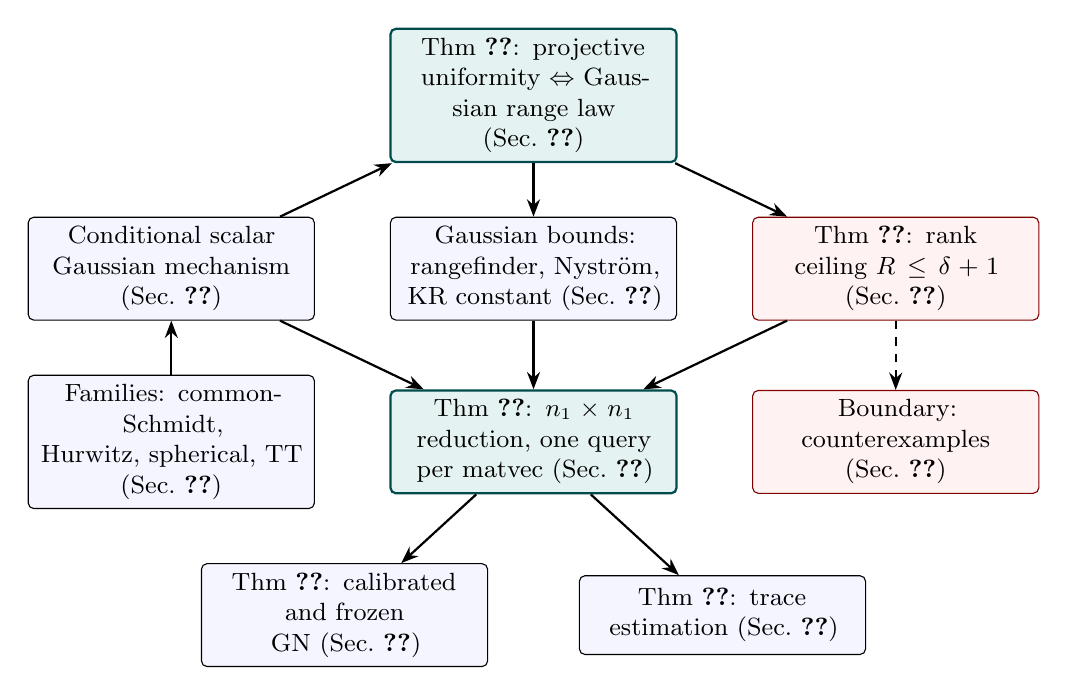
\begin{tikzpicture}[
  box/.style={draw,rounded corners=2pt,align=center,font=\small,
              minimum height=10mm,text width=34mm,fill=blue!4},
  key/.style={box,fill=teal!10,draw=teal!60!black,thick},
  lim/.style={box,fill=red!5,draw=red!50!black},
  arr/.style={-{Stealth[length=2.2mm]},thick}]
\node[key] (iff) at (0,0) {Thm~\ref{mthm:iff}: projective\\ uniformity $\Leftrightarrow$
  Gaussian range law\\ (Sec.~\ref{sec:iff})};
\node[box] (mech) at (-4.6,-2.2) {Conditional scalar\\ Gaussian mechanism\\
  (Sec.~\ref{sec:mechanism})};
\node[box] (fam) at (-4.6,-4.4) {Families: common-Schmidt,\\ Hurwitz, spherical,
  TT\\ (Sec.~\ref{sec:families})};
\node[lim] (ceil) at (4.6,-2.2) {Thm~\ref{mthm:ceiling}: rank\\ ceiling
  $R\le\delta+1$\\ (Sec.~\ref{sec:ceiling})};
\node[box] (bounds) at (0,-2.2) {Gaussian bounds:\\ rangefinder, Nystr\"om,\\
  KR constant (Sec.~\ref{sec:bounds})};
\node[key] (red) at (0,-4.4) {Thm~\ref{mthm:reduction}: $n_1\times n_1$\\
  reduction, one query\\ per matvec (Sec.~\ref{sec:reduction})};
\node[box] (gn) at (-2.4,-6.6) {Thm~\ref{mthm:gn}: calibrated\\ and frozen GN
  (Sec.~\ref{sec:gn})};
\node[box] (trace) at (2.4,-6.6) {Thm~\ref{mthm:trace}: trace\\ estimation
  (Sec.~\ref{sec:trace})};
\node[lim] (limits) at (4.6,-4.4) {Boundary:\\ counterexamples\\
  (Sec.~\ref{sec:limits})};
\draw[arr] (fam) -- (mech);
\draw[arr] (mech) -- (iff);
\draw[arr] (iff) -- (bounds);
\draw[arr] (iff) -- (ceil);
\draw[arr] (mech) -- (red);
\draw[arr] (ceil) -- (red);
\draw[arr] (red) -- (gn);
\draw[arr] (red) -- (trace);
\draw[arr] (bounds) -- (red);
\draw[arr,dashed] (ceil) -- (limits);
\end{tikzpicture}
\caption{Roadmap. Teal boxes are the two structural theorems; red boxes mark
the limits of the class.}
\label{fig:roadmap}
\end{figure}
\section{Range-determined outputs and the exact criterion}\label{sec:iff}

\subsection{Which outputs are range-determined}

The basic identity is that a fixed linear map $B$ with $BV_\perp=0$, where
$[V\ V_\perp]$ is orthogonal, satisfies $B=BVV^\T$, hence
\begin{equation}\label{eq:basic}
 \range(B\Omega)=BV\,\range(V^\T\Omega).
\end{equation}

\begin{lemma}[Catalogue of range-determined outputs]\label{lem:catalogue}
The following outputs are range-determined on $S$ in the sense of
Definition~\ref{def:rangedet}.
\begin{enumerate}[label=\textup{(\alph*)}]
\item The rangefinder projector $P_{A\Omega}$, where $S$ is the row space of $A$.
\item The joint ranges of $Y_j=(AA^\T)^jA\Omega$, $j=0,\ldots,s$, and of
      their concatenation $[Y_0\ \cdots\ Y_s]$; for $A\succeq0$ with range $S$,
      the ranges of $f_j(A)\Omega$ and their concatenation whenever $f_j(0)=0$.
\item The PSD Nystr\"om approximation
      $C=A\Omega(\Omega^\T A\Omega)^\dagger\Omega^\T A$ for $A\succeq0$ with range
      $S$, and its best rank-$r$ truncation $C_r$ (with a fixed measurable
      tie-breaking rule).
\item Generalized Nystr\"om $\widehat A_\GN=A\Omega(\Psi^\T A\Omega)^\dagger\Psi^\T A$
      with a left sketch $\Psi$ independent of $\Omega$ and injective on
      $\range(A\Omega)$ almost surely (e.g. dense Gaussian with $p\ge k$
      columns).
\end{enumerate}
\end{lemma}

\begin{proof}
\emph{Rangefinder.} $A$ annihilates $S^\perp$, so \eqref{eq:basic} applies,
and $AV$ is injective.

\emph{Powered ranges.} Each $(AA^\T)^jA$ and each $f_j(A)$ with $f_j(0)=0$ annihilates
$S^\perp$. The range of the concatenation is
$\sum_jB_jV\range(V^\T\Omega)$.

\emph{PSD Nystr\"om.} With $M=A^{1/2}\Omega$, the identity
$M(M^\T M)^\dagger M^\T=P_{\range M}$ gives
\begin{equation}\label{eq:nys-projector}
 C=A^{1/2}P\,A^{1/2},\qquad P=P_{\range(A^{1/2}\Omega)},
\end{equation}
and $\range(A^{1/2}\Omega)=A^{1/2}V\range(V^\T\Omega)$. The truncation is a
measurable function of $C$.

\emph{Generalized Nystr\"om.} Let $Q$ be an orthonormal basis of
$\range Y$, $Y=A\Omega=QT$ with $T$ of full row rank. If $\Psi^\T Q$ has full
column rank then $(\Psi^\T QT)^\dagger=T^\dagger(\Psi^\T Q)^\dagger$, so
\begin{equation}\label{eq:gn-q}
 \widehat A_\GN=Q(\Psi^\T Q)^\dagger\Psi^\T A,
\end{equation}
which depends on $\Omega$ only through $\range Y=AV\range(V^\T\Omega)$.
\end{proof}

Outputs that are \emph{not} range-determined include the sketch Gram matrix
$\Omega^\T A^\T A\Omega$, embedding distortions
$\sup_{x\in S}|\norm{\Omega^\T x}^2/\norm x^2-1|$, raw inverse-Gram moments, raw QR
factors, stopping rules or regularization chosen from unnormalized sketch
singular values, Krylov spaces that include the raw columns of $\Omega$, and
generalized Nystr\"om with an unnormalized structured left sketch. Figure~\ref{fig:schematic}
summarizes the distinction.

\begin{figure}[t]
\centering
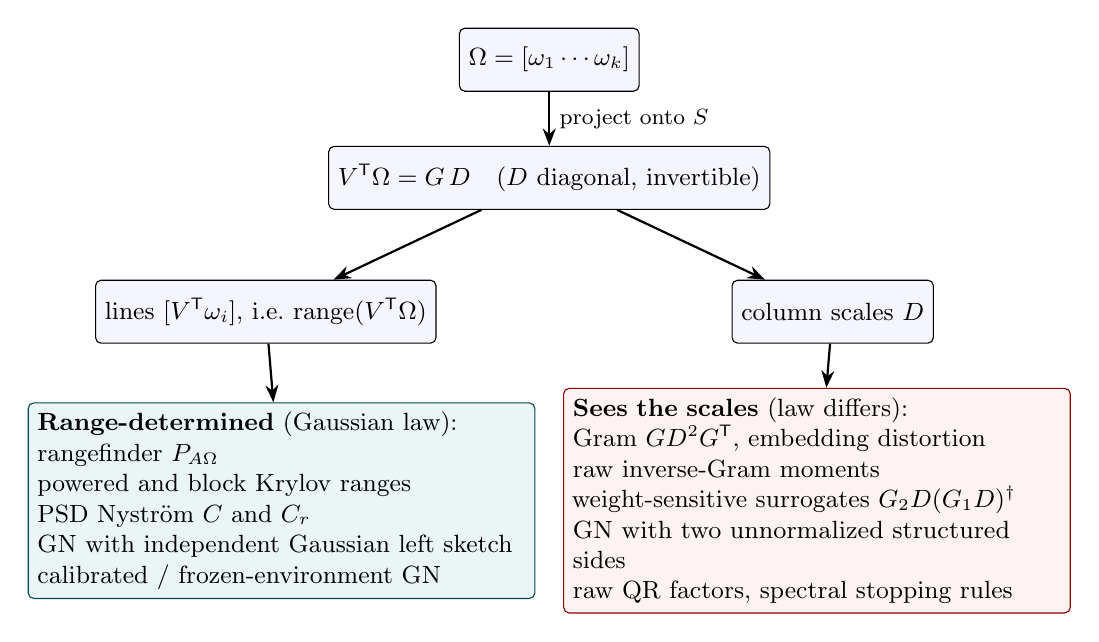
\begin{tikzpicture}[
  n/.style={draw,rounded corners=2pt,align=center,font=\small,fill=blue!4,
            minimum height=8mm},
  ok/.style={draw=teal!60!black,rounded corners=2pt,align=left,font=\small,
            fill=teal!8,text width=62mm},
  no/.style={draw=red!55!black,rounded corners=2pt,align=left,font=\small,
            fill=red!5,text width=62mm},
  arr/.style={-{Stealth[length=2.2mm]},thick}]
\node[n] (om) at (0,0) {$\Omega=[\omega_1\cdots\omega_k]$};
\node[n] (proj) at (0,-1.5) {$V^\T\Omega=G\,D$\quad
   ($D$ diagonal, invertible)};
\node[n] (lines) at (-3.6,-3.2) {lines $[V^\T\omega_i]$, i.e.\
   $\range(V^\T\Omega)$};
\node[n] (scales) at (3.6,-3.2) {column scales $D$};
\node[ok] (good) at (-3.4,-5.6) {\textbf{Range-determined} (Gaussian law):\\
  rangefinder $P_{A\Omega}$\\ powered and block Krylov ranges\\
  PSD Nystr\"om $C$ and $C_r$\\ GN with independent Gaussian left sketch\\
  calibrated / frozen-environment GN};
\node[no] (bad) at (3.4,-5.6) {\textbf{Sees the scales} (law differs):\\
  Gram $GD^2G^\T$, embedding distortion\\ raw inverse-Gram moments\\
  weight-sensitive surrogates $G_2D(G_1D)^\dagger$\\
  GN with two unnormalized structured sides\\ raw QR factors, spectral stopping rules};
\draw[arr] (om) -- node[right,font=\footnotesize]{project onto $S$} (proj);
\draw[arr] (proj) -- (lines);
\draw[arr] (proj) -- (scales);
\draw[arr] (lines) -- (good);
\draw[arr] (scales) -- (bad);
\end{tikzpicture}
\caption{What is and is not range-determined. Under the criterion of
Theorem~\ref{mthm:iff} the lines have their Gaussian law; the scales $D$ do not.
Outputs on the left have exactly the dense-Gaussian law; outputs on the right
depend on $D$ and generally do not.}
\label{fig:schematic}
\end{figure}

\subsection{Proof of the criterion}

\begin{proof}[Proof of Theorem~\ref{mthm:iff}]
(iii)$\Rightarrow$(i). For a dense Gaussian probe $\gamma$,
$V^\T\gamma\sim N(0,I_R)$ is nonzero almost surely, and its line is
uniformly distributed on $\RP^{R-1}$, i.e.\ has the unique $O(R)$-invariant
probability law, by rotation invariance. Under (iii), the lines
$[V^\T\omega_1],\ldots,[V^\T\omega_k]$ are therefore iid with the same law as
$[V^\T\gamma_1],\ldots,[V^\T\gamma_k]$. The subspace
$\range(V^\T\Omega)=\sum_i[V^\T\omega_i]$ is a Borel function of this
$k$-tuple of lines. So the two ranges have the same law in $\mathcal G_R$,
for every $k$. By Definition~\ref{def:rangedet} and independence of the
auxiliary randomness, every range-determined output has its Gaussian law.

(i)$\Rightarrow$(ii). Take $k=1$ in \eqref{eq:basic}:
$\range(A\omega)=AV\range(V^\T\omega)$.

(ii)$\Rightarrow$(iii). Let $A$ have row space $S$. Then $AV$ is injective and
$A\omega=AV(V^\T\omega)$. For the Gaussian probe, $\range(A\gamma)$ is a line
almost surely. Equality of laws forces $\range(A\omega)$ to be a line almost
surely, hence $V^\T\omega\ne0$ almost surely. The map
$\varphi\colon\RP^{R-1}\to\RP^{N_L-1}$, $\ell\mapsto AV\ell$, is continuous
and injective on a compact space, hence a homeomorphism onto its compact
image. Since $\varphi([V^\T\omega])$ and $\varphi([V^\T\gamma])$ have the same
law, applying the Borel map $\varphi^{-1}$ on the image shows that
$[V^\T\omega]$ and $[V^\T\gamma]$ have the same law, the uniform one.
The argument used only one $A$; since (iii) does not involve $A$, the
equivalence holds for one and for every such $A$.
\end{proof}

\begin{corollary}[Coupling and joint statements]\label{cor:coupling}
Under the conditions of Theorem~\ref{mthm:iff}, on a suitable probability space
$V^\T\Omega=GD$, where $G\in\R^{R\times k}$ has iid $N(0,1)$ entries and
$D$ is an almost surely invertible diagonal matrix. Consequently, for every
finite family of fixed maps $B_j$ annihilating $S^\perp$, jointly,
$\range(B_j\Omega)=\range(B_jVG)$ and the range of any horizontal concatenation
equals that of the corresponding concatenation with $\Gamma=VG+V_\perp G_\perp$,
a dense Gaussian matrix.
\end{corollary}

\begin{proof}
Put $u=V^\T\omega\ne0$ and $\theta=u/\norm u$. Draw an independent uniform sign
$\epsilon$ and an independent radius $\rho\sim\chi_R$. Since $[\theta]$ is
uniform on $\RP^{R-1}$ and $\epsilon$ is an independent symmetric sign,
$\epsilon\theta$ is uniform on the sphere; with the independent radius,
$g=\epsilon\rho\,\theta\sim N(0,I_R)$. Then $u=(\epsilon\norm u/\rho)\,g$.
Do this independently for each column. The joint statement follows from
$B_j=B_jVV^\T$ and $B_j\Gamma=B_jVG$; an invertible right factor, or a block
diagonal one with a copy of $D$ per block, preserves column ranges.
\end{proof}

In this coupling $D$ need not be independent of $G$. Under the conditional
Gaussian mechanism of Section~\ref{sec:mechanism} it is.
\section{A checkable sufficient mechanism}\label{sec:mechanism}

Projective uniformity is the exact condition, but it is rarely checked
directly. The following mechanism is.

\begin{definition}[Conditional scalar Gaussianity]\label{def:csg}
A probe $\omega$ is \emph{conditionally scalar Gaussian on $S$} if there is a
$\sigma$-field $\mathcal F$ and an $\mathcal F$-measurable random variable $w$
with $w>0$ almost surely such that
\begin{equation}\label{eq:criterion}
 V^\T\omega\mid\mathcal F\ \sim\ N(0,wI_R).
\end{equation}
For a sketch we require that the pairs $(\omega_i,\mathcal F_i)$ be
independent across columns $i$.
\end{definition}

\begin{theorem}[Mechanism]\label{thm:mechanism}
Assume Definition~\ref{def:csg}, including independence of the pairs
$(\omega_i,\mathcal F_i)$ across $i$. Then $g_i=V^\T\omega_i/\sqrt{w_i}$ are iid
$N(0,I_R)$ and the family $(g_i)$ is independent of $(w_i)$. Hence
\begin{equation}\label{eq:GD}
 V^\T\Omega=GD,\qquad G\ \text{iid }N(0,1),\quad
 D=\diag(\sqrt{w_1},\ldots,\sqrt{w_k}),\quad G\perp D,
\end{equation}
and the conditions of Theorem~\ref{mthm:iff} hold.
\end{theorem}

\begin{proof}
Conditionally on $\mathcal F_i$, $g_i\sim N(0,I_R)$, a law that does not
depend on $\mathcal F_i$. For Borel $E$ and $F\in\mathcal F_i$,
$\Prob\{g_i\in E,\,F\}=\E[\mathbf 1_F\Prob(g_i\in E\mid\mathcal F_i)]
=\Prob\{N(0,I_R)\in E\}\Prob(F)$. So $g_i$ is independent of $\mathcal F_i$,
in particular of $w_i$. Independence of the pairs across $i$ gives the joint
statement. Finally $V^\T\omega_i=\sqrt{w_i}\,g_i$ is nonzero almost surely and
$[V^\T\omega_i]=[g_i]$ is uniform on $\RP^{R-1}$.
\end{proof}

The column-independence hypothesis is used exactly once, in the joint
statement. It matters for designs that share randomness between columns,
such as block tensor-train sketches with shared cores; those require a
separate joint argument. (Frozen environments, used later, are handled by
conditioning on the shared environment, Remark~\ref{rem:frozen-range}.)

\begin{remark}[The mechanism is strictly stronger than the criterion]
\label{rem:stronger}
Equation~\eqref{eq:criterion} forces $V^\T\omega=\sqrt w\,g$ with $g$
independent of $w$. Hence $\norm{V^\T\omega}$ is a scale mixture of $\chi_R$
and is independent of the direction. A probe uniform on the unit sphere of
$S$ has constant radius and violates \eqref{eq:criterion}, and so does
$\rho(\theta)\theta$ with a direction-dependent radius. Both satisfy
Theorem~\ref{mthm:iff}.
\end{remark}

\begin{corollary}[Nonzero rescalings, spherical factors]\label{cor:spherical}
If $\omega$ satisfies the conditions of Theorem~\ref{mthm:iff} and $c$ is a
random scalar that is nonzero almost surely, possibly dependent on $\omega$,
then $c\,\omega$ satisfies them too. In particular, if a Gaussian product
probe $g_1\otimes\cdots\otimes g_q$ satisfies them, so does the spherical
product probe $\bigotimes_j\rho_j g_j/\norm{g_j}$ for any fixed radii
$\rho_j>0$.
\end{corollary}

\begin{proof}
$[V^\T(c\omega)]=[V^\T\omega]$, and $V^\T(c\omega)\ne0$ almost surely. The
spherical probe is $c\,\omega$ with $c=\prod_j\rho_j/\norm{g_j}$.
\end{proof}

\begin{remark}[The complex case]\label{rem:complex}
Everything above holds over $\C$ with $V^*$ in place of $V^\T$, unitary
invariance in place of orthogonal invariance, the complex projective space
$\mathbb{CP}^{R-1}$, and the complex Grassmannian. The mechanism becomes
$V^*\omega\mid\mathcal F\sim\mathcal{CN}(0,wI_R)$. Complex common-Schmidt
product supports and the single-core common-Schmidt tensor-train family are
covered after replacing orthonormality by Hermitian orthonormality. For other
supports the Hermitian conditional covariance must be checked directly. The
real Hurwitz test $\sym(M_a^\T M_c)=0$ does not imply $M_a^*M_c=0$, so its
real examples do not automatically transfer to complex factors. Spherical
factors follow from the complex version of Corollary~\ref{cor:spherical}. The only
change in the Gaussian constants of Section~\ref{sec:bounds} is the
pseudoinverse moment: for an $r\times k$ standard complex Gaussian $G_1$
($\E|g_{ij}|^2=1$) and $k>r$, $\E\norm{G_1^\dagger}_\F^2=r/(k-r)$, the
complex inverse-Wishart mean.
\end{remark}
\section{Certified families}\label{sec:families}

We use one elementary fact repeatedly: \emph{a nonzero real polynomial on
$\R^d$ has a Lebesgue-null zero set.} (Induction on $d$: outside the null set
of lower variables where all coefficients of the top variable vanish, a
nonzero univariate polynomial has finitely many roots; Fubini finishes.)
Consequently a polynomial in Gaussian variables that is nonzero with
positive probability is nonzero almost surely, and a polynomial identity that
holds almost surely holds identically.

\subsection{Gaussian product probes}

Let $\omega=g\otimes h$ with $g\sim N(0,I_{n_1})$ and $h=h_2\otimes\cdots\otimes h_q$,
where all factors are independent standard Gaussian vectors, and put
$n'=\prod_{j\ge2}n_j$. Reshape $v\in\R^{n_1}\otimes\R^{n'}$ as
$M_v\in\R^{n_1\times n'}$ so that $v^\T(g\otimes h)=g^\T M_vh$. Let
$L_h=I_{n_1}\otimes h\in\R^{N\times n_1}$, so that $L_hg=g\otimes h$ and
$L_h^\T v=M_vh$. Conditionally on $h$, $V^\T\omega=V^\T L_hg$ is centered
Gaussian with covariance $V^\T L_hL_h^\T V$, whose $(a,c)$ entry is
$h^\T M_a^\T M_ch$, where $M_a=M_{u_a}$ for the columns $u_a$ of $V$.

\begin{definition}[Conditionally Gaussian product class]\label{def:cgp}
The support $S$ belongs to the \emph{conditionally Gaussian product class}
if $V^\T L_hL_h^\T V=w(h)I_R$ with $w(h)>0$ for almost every $h$; that is,
\eqref{eq:criterion} holds with $\mathcal F=\sigma(h_2,\ldots,h_q)$. The same
definition applies with any other factor in the role of $g$.
\end{definition}

\begin{proposition}[Common-Schmidt family, any order]\label{prop:schmidt}
Suppose the orthonormal basis of $S$ has the form
\begin{equation}\label{eq:schmidt}
 u_a=\sum_{b=1}^{\ell}\sqrt{\lambda_b}\,e_{a,b}\otimes f_b,\qquad a=1,\ldots,R,
\end{equation}
where $\lambda_b>0$, $\sum_b\lambda_b=1$, the \emph{entire} family
$\{e_{a,b}\}_{a,b}\subset\R^{n_1}$ is orthonormal, and $f_1,\ldots,f_\ell$ are
orthonormal tensors in $\R^{n'}$ (not necessarily of rank one). Then $S$
belongs to the conditionally Gaussian product class with
\begin{equation}\label{eq:wkr}
 w(h)=\sum_{b}\lambda_b\langle f_b,h\rangle^2 .
\end{equation}
Necessarily $R\ell\le n_1$ and $\ell\le n'$.
\end{proposition}

\begin{proof}
$\langle u_a,g\otimes h\rangle=\sum_b\sqrt{\lambda_b}\langle e_{a,b},g\rangle
\langle f_b,h\rangle$. The coefficients $\langle e_{a,b},g\rangle$ are iid
$N(0,1)$, and different $a$ use disjoint sets of them, so the conditional
covariance is $\delta_{ac}\sum_b\lambda_b\langle f_b,h\rangle^2$. Rank-one
tensors span $\R^{n'}$, so $h\mapsto\langle f_b,h\rangle$ is a nonzero
polynomial in the factor coordinates; hence $w(h)>0$ almost surely. The
dimension bounds follow from orthonormality.
\end{proof}

Choosing coordinate vectors for $e_{a,b}$ and $f_b$ and any positive
eigenvalues $\mu_a$ gives inputs $A=\sum_a\mu_au_au_a^\T$ in the class, with no
restriction on spectral decay. For $\ell=1$ this is $A=A_1\otimes ff^\T$ with a
fixed unit tensor $f$ and PSD $A_1$ on the first factor; for $\ell>1$ the
eigenvectors are entangled. The Schmidt weights $\lambda_b$ describe
eigenvectors and must not be confused with the eigenvalues $\mu_a$.

\subsection{An algebraic test for two factors, and a Hurwitz family}

\begin{proposition}[Algebraic test]\label{prop:test}
Let $q=2$ and let $u_1,\ldots,u_R$ be orthonormal. Then $S$ belongs to the
conditionally Gaussian product class if and only if there is $S_0\succeq0$
with $\tr S_0=1$ such that
\begin{equation}\label{eq:test}
 \sym(M_a^\T M_c)=\delta_{ac}S_0\qquad(1\le a,c\le R),
 \qquad \sym M=\tfrac12(M+M^\T).
\end{equation}
Then $w(h)=h^\T S_0h$. Equivalently, in basis-free form,
$M_v^\T M_v=\norm v^2S_0$ for every $v\in S$.
\end{proposition}

\begin{proof}
The conditional covariance entry $h^\T M_a^\T M_ch$ depends only on the
symmetric part of $M_a^\T M_c$, which proves sufficiency. Conversely, if
$h^\T(M_a^\T M_c-\delta_{ac}\,M_1^\T M_1)h=0$ almost surely, the polynomial
vanishes identically, so its symmetric coefficient matrix vanishes; put
$S_0=\sym(M_1^\T M_1)=M_1^\T M_1\succeq0$, with $\tr S_0=\norm{M_1}_\F^2=1$.
Positivity of $h^\T S_0h$ almost surely follows because $S_0\ne0$. For the
basis-free form expand $M_v=\sum_ac_aM_a$; the cross terms are the symmetric
parts in \eqref{eq:test}. Conversely, apply the basis-free identity to $u_a$,
$u_c$ and $u_a+u_c$ and polarize.
\end{proof}

\begin{example}[A family outside the common-Schmidt form]\label{ex:hurwitz}
Let $n_1=n_2=2$ and
\[
 M_1=\tfrac1{\sqrt2}\begin{bmatrix}1&0\\0&1\end{bmatrix},\qquad
 M_2=\tfrac1{\sqrt2}\begin{bmatrix}0&-1\\1&0\end{bmatrix}.
\]
Then $M_1^\T M_1=M_2^\T M_2=I_2/2$ and $\sym(M_1^\T M_2)=0$, so
\eqref{eq:test} holds with $S_0=I_2/2$. Both $M_a$ have Schmidt rank two, and a
common-Schmidt representation with $R=\ell=2$ would need four orthonormal
vectors in $\R^2$. More generally, when $S_0=I_{n_2}/n_2$ the matrices
$L_a=\sqrt{n_2}M_a$ satisfy $L_a^\T L_c+L_c^\T L_a=2\delta_{ac}I$, equivalently
$\norm{\sum_ax_aL_ay}^2=\norm x^2\norm y^2$: these are the classical
Hurwitz--Radon sum-of-squares identities \cite{LMO}. Square families exist
exactly up to the Radon--Hurwitz number, e.g.\ $R=4$ for $n_1=n_2=4$
(quaternions) and $R=8$ for $n_1=n_2=8$ (octonions). The identities are
classical; here they provide a certificate of exact Gaussian range laws.
\end{example}

\begin{remark}[Exchanging the factors]\label{rem:mirror}
Conditioning on $g$ instead of $h$ gives the mirror test
$\sym(M_aM_c^\T)=\delta_{ac}S_0'$ with $w=g^\T S_0'g$; for example
$u_a=f\otimes e_a$. For two factors the certified class is the union of the two
tests; at higher order any single factor may be left unconditioned.
\end{remark}

\subsection{A single-core tensor-train family}

Let there be $q$ sites with physical dimensions $d_j$, bond dimensions
$\chi_0=\chi_q=1$ and $\chi_j=\chi$ for $0<j<q$, and independent cores
$H_j\in\R^{\chi_{j-1}\times d_j\times\chi_j}$ with iid $N(0,1)$ entries. Define
\begin{equation}\label{eq:tt}
 \omega(i_1,\ldots,i_q)=\chi^{-(q-1)/2}\sum_{\alpha_1,\ldots,\alpha_{q-1}}
 \prod_{j=1}^qH_j(\alpha_{j-1},i_j,\alpha_j),\qquad\alpha_0=\alpha_q=1,
\end{equation}
with all cores regenerated independently for each column \cite{RR,CDF}.
Averaging a product of two entries forces all physical and bond indices to
match; the $\chi^{q-1}$ surviving bond paths cancel the normalization, so
$\E\omega\omega^\T=I$. Fix a site $t$ and condition on the other cores.
After a fixed permutation of tensor factors,
\begin{equation}\label{eq:tt-cut}
 \omega=\sum_{\alpha=1}^{\chi_{t-1}}\sum_{\beta=1}^{\chi_t}
 C_{\alpha\beta}\otimes g_{\alpha\beta},\qquad g_{\alpha\beta}=H_t(\alpha,:,\beta),
\end{equation}
where the tensors $C_{\alpha\beta}$ on the other sites absorb the normalization
and the $g_{\alpha\beta}$ are iid $N(0,I_{d_t})$.

\begin{proposition}[Single-core common-Schmidt family]\label{prop:tt}
Suppose $S$ has an orthonormal basis
$u_a=\sum_{b=1}^\ell\sqrt{\lambda_b}\,X_b\otimes\phi_{a,b}$, with $\lambda_b>0$,
$\sum_b\lambda_b=1$, orthonormal tensors $X_b$ on the other sites, and the
entire family $\{\phi_{a,b}\}$ orthonormal in $\R^{d_t}$. Then
\eqref{eq:criterion} holds conditionally on the other cores, with
$w=\sum_{\alpha,\beta,b}\lambda_b\langle X_b,C_{\alpha\beta}\rangle^2>0$ almost
surely. Necessarily $R\ell\le d_t$.
\end{proposition}

\begin{proof}
By \eqref{eq:tt-cut},
$\langle u_a,\omega\rangle=\sum_{\alpha,\beta,b}\sqrt{\lambda_b}
\langle X_b,C_{\alpha\beta}\rangle\langle\phi_{a,b},g_{\alpha\beta}\rangle$,
which is conditionally Gaussian with covariance
$\sum_{\alpha\beta}\sum_{b,c}\sqrt{\lambda_b\lambda_c}\langle X_b,C_{\alpha\beta}\rangle
\langle X_c,C_{\alpha\beta}\rangle\langle\phi_{a,b},\phi_{a',c}\rangle=\delta_{aa'}w$.
The function $w$ is a nonnegative polynomial in the other cores, and
$\E w=\E\langle u_a,\omega\rangle^2=1$ by isotropy, so $w$ is not identically
zero and is positive almost surely.
\end{proof}

Orthonormal product tensors $X_b$ and distinct coordinate vectors $\phi_{a,b}$
give concrete PSD inputs with Gaussian Nystr\"om laws, for every $\chi$ and $q$.
At fixed $d_t$ this construction has $R\le d_t/\ell$; conditioning on one core
always bounds the conditional covariance rank by $d_t\chi_{t-1}\chi_t$.
\section{The rank ceiling}\label{sec:ceiling}

The families of Section~\ref{sec:families} all have small rank. This is not an
artifact of the constructions. We use the following standard fact
\cite[Corollary~6.11]{Lee}: \emph{if $f\colon M\to N$ is a $C^1$ map between
smooth manifolds with $\dim M<\dim N$, then $f(M)$ has measure zero in $N$}
(for any smooth positive density on $N$).

\begin{proof}[Proof of Theorem~\ref{mthm:ceiling}]
Let $\Sigma=\{x_1\otimes\cdots\otimes x_q\}$ be the cone of rank-one tensors and
$M=S^{n_1-1}\times\cdots\times S^{n_q-1}$, a manifold of dimension $\delta$.
Every nonzero $x\in\Sigma$ equals $c\,\xi_1\otimes\cdots\otimes\xi_q$ with $c\ne0$
and $(\xi_j)\in M$. Let $U\subseteq M$ be the open set where
$V^\T(\xi_1\otimes\cdots\otimes\xi_q)\ne0$, and
$\varphi\colon U\to\RP^{R-1}$, $\xi\mapsto[V^\T(\xi_1\otimes\cdots\otimes\xi_q)]$,
a smooth map.

(i) Under Theorem~\ref{mthm:iff}, $V^\T\omega\ne0$ almost surely and
$[V^\T\omega]=\varphi(\xi)\in\varphi(U)$, where $\xi$ is the normalized factor
tuple. If $\delta<R-1$, then $\varphi(U)$ is null in $\RP^{R-1}$, contradicting
uniformity of $[V^\T\omega]$. Hence $R\le\delta+1$. Under conditional scalar
Gaussianity the conditions of Theorem~\ref{mthm:iff} hold
(Theorem~\ref{thm:mechanism}), so the same bound applies. Attainment is
Example~\ref{ex:hook} below.

(ii) Fix $k<R$. For the Gaussian sketch, $\range(V^\T\Gamma)$ lies in
$\Gr(k,R)$ almost surely and has the $O(R)$-invariant law, which has a smooth
positive density. If the structured range has the same law, it is
$k$-dimensional almost surely; then all columns are nonzero, their
normalized factor tuples lie in $U$, and
$\range(V^\T\Omega)=\Phi(\xi^{(1)},\ldots,\xi^{(k)})$, where
$\Phi(\xi^{(1)},\ldots,\xi^{(k)})=\varphi(\xi^{(1)})+\cdots+\varphi(\xi^{(k)})$ is
smooth on the open subset of $U^k$ where these lines are independent. That
subset has dimension $k\delta$ and $\dim\Gr(k,R)=k(R-k)$. If $R>k+\delta$ then
$k\delta<k(R-k)$, the image of $\Phi$ is null, and we reach a contradiction.
Hence $R\le k+\delta$. Nothing about the joint law of the columns was used.

(iii) In the conditionally Gaussian product class,
$V^\T L_hL_h^\T V=w(h)I_R$ with $w(h)>0$, so the $R\times n_1$ matrix $V^\T L_h$
has rank $R$, and $R\le n_1$.
\end{proof}

\begin{example}[The ceiling is attained]\label{ex:hook}
Let $z_0\in\R$ and $z_j\in\R^{n_j-1}$, $j=1,\ldots,q$, be independent standard
Gaussian, and put
\[
 x_1=(z_1,z_0),\qquad x_j=(z_j/z_0,\,1)\quad(j\ge2),\qquad
 \omega=x_1\otimes\cdots\otimes x_q .
\]
Let $H$ be the ``hook'' of multi-indices $(i_1,\ldots,i_q)$ with at most one
coordinate $i_j<n_j$ and all others equal to their maximum. Then $|H|=\delta+1$,
$\omega(n_1,\ldots,n_q)=z_0$, the entries with $i_1<n_1$ are the coordinates
of $z_1$, and the entries with $i_j<n_j$ for $j\ge2$ equal
$z_0\cdot z_j(i_j)/z_0=z_j(i_j)$. With $V$ the coordinate isometry onto
$\R^H$, $V^\T\omega=(z_0,z_1,\ldots,z_q)\sim N(0,I_{\delta+1})$: the mechanism
holds with $w\equiv1$ on a support of dimension $\delta+1$. The factors share
$z_0$ and are therefore dependent; the ratios in the later factors are
heavy-tailed. This attains the ceiling under the arbitrary joint factor laws
allowed in Theorem~\ref{mthm:ceiling}(i), and does not establish attainment
for independent factors. For independent Gaussian factors and the
conditional mechanism, part~(iii) gives the smaller ceiling $n_1$.
\end{example}

\begin{remark}[What the ceiling means]\label{rem:window}
With base dimension two ($n_j=2$, $n=2^q$) we get $\delta=q$ and $R\le\log_2n+1$;
for $n=2^{20}$, at most $21$. For $k\ge R$ the Gaussian rangefinder is exact
and the question is vacuous. So the class-specific theorems of
Sections~\ref{sec:bounds}--\ref{sec:trace} have content only in the window
$r+1<k<R\le\delta+1$, and for the conditionally Gaussian product class in
$r+1<k<R\le n_1$. They are exact identifications, and they should be framed
as such: the class is explicit and checkable, but it is not a large class of
inputs.
\end{remark}

\begin{remark}[Tensor trains: growing rank is not excluded]\label{rem:tt-open}
The probe \eqref{eq:tt} lies in the tensor-train variety $\mathcal T_\chi$ of
tensors with TT ranks at most $\chi$. It is the image of the core space, of
dimension $D_\chi=\sum_j\chi_{j-1}d_j\chi_j$, under a polynomial map. The
proof of part~(i), applied to this map (whose line is unchanged when the first
core is multiplied by a nonzero scalar, so the effective parameter count is
$D_\chi-1$), gives $R\le D_\chi$ under the conditions of
Theorem~\ref{mthm:iff}; with the semialgebraic dimension of $\mathcal T_\chi$
in place of the parameter count, $R\le\dim\mathcal T_\chi\le D_\chi$. This bound grows with $\chi$ and $q$, so
the dimension count does \emph{not} rule out Gaussian tensor-train probes with
exact Gaussian range laws on supports of growing rank. Proposition~\ref{prop:tt}
is the only tensor-train family proved here, and it has $R\le d_t/\ell$ at fixed
physical dimension. We make no claim of a growing-rank tensor-train theorem;
see Section~\ref{sec:open}.
\end{remark}
\section{Gaussian approximation bounds on the class}\label{sec:bounds}

Equality of laws transfers every correctly scoped Gaussian theorem about a
range-determined output. We give complete proofs of the two most used
bounds, classical in the Gaussian setting \cite{HMT,TYUCpsd}, to make visible
that random column scales and tensor dimensions contribute no extra factor.

\begin{lemma}[Gaussian pseudoinverse moment]\label{lem:inverse}
Let $G_1\in\R^{r\times k}$ have iid $N(0,1)$ entries and $k>r+1$. Then
$\E\norm{G_1^\dagger}_\F^2=r/(k-r-1)$.
\end{lemma}

\begin{proof}
The rows are independent almost surely and
$\norm{G_1^\dagger}_\F^2=\tr(G_1G_1^\T)^{-1}$. By the Schur complement, the
$i$-th diagonal entry of $(G_1G_1^\T)^{-1}$ is the reciprocal of the squared
distance from row $i$ to the span of the other $r-1$ rows. Conditionally on
those rows this squared distance is $\chi^2_\nu$ with $\nu=k-r+1$, and
$\E(\chi^2_\nu)^{-1}=1/(\nu-2)$ by the gamma integral. Sum over $i$.
\end{proof}

\begin{theorem}[Rangefinder]\label{thm:rf}
Let the row space $S$ of $A$ satisfy Theorem~\ref{mthm:iff}, and let $r+1<k\le R$.
Then $P_{A\Omega}$ has its Gaussian law and
\begin{equation}\label{eq:rf}
 \E\norm{A-P_{A\Omega}A}_\F^2\le\Bigl(1+\frac r{k-r-1}\Bigr)\tau^{(2)}_r(A).
\end{equation}
If $k\ge R$ the rangefinder is exact almost surely.
\end{theorem}

\begin{proof}
By Lemma~\ref{lem:catalogue}(a) and Theorem~\ref{mthm:iff} we may replace
$V^\T\Omega$ by a Gaussian $G$.

\emph{Step 1: construct a candidate inside the sketch range.}
With the compact SVD $A=U\Sigma V^\T$, split
$G=[G_1;G_2]$ after $r$ rows and $\Sigma=\diag(\Sigma_1,\Sigma_2)$. The range of
$Y=U\Sigma G$ contains the columns of
\[
 YG_1^\dagger
 =U\begin{bmatrix}\Sigma_1\\\Sigma_2G_2G_1^\dagger\end{bmatrix}.
\]
Using this matrix times the leading right singular vectors as a candidate,
and since orthogonal projection is optimal among matrices with columns in
$\range Y$, we obtain
\[
 \norm{A-P_YA}_\F^2
 \le\norm{\Sigma_2}_\F^2+\norm{\Sigma_2G_2G_1^\dagger}_\F^2.
\]

\emph{Step 2: average the cross term.}
Conditionally on $G_1$, $G_2$ is an independent Gaussian matrix and
\[
 \E\bigl[\norm{\Sigma_2G_2G_1^\dagger}_\F^2\mid G_1\bigr]
 =\norm{\Sigma_2}_\F^2\norm{G_1^\dagger}_\F^2.
\]
Apply Lemma~\ref{lem:inverse}. For $k\ge R$, $G$ has full row rank almost
surely.
\end{proof}

\begin{theorem}[PSD Nystr\"om, including fixed rank]\label{thm:nys}
Let $A\succeq0$ have range $S$ satisfying Theorem~\ref{mthm:iff}. Then
$C=A\Omega(\Omega^\T A\Omega)^\dagger\Omega^\T A$ and its best rank-$r$
truncation $C_r$ have their Gaussian laws, and for $r+1<k\le R$,
\begin{equation}\label{eq:nys}
 \E\tr(A-C)\le\E\tr(A-C_r)\le\Bigl(1+\frac r{k-r-1}\Bigr)\tau_r(A).
\end{equation}
If $k\ge R$ then $C=A$ almost surely and $C_r$ is a best rank-$r$ approximation.
\end{theorem}

\begin{proof}
By \eqref{eq:nys-projector}, $0\preceq C_r\preceq C\preceq A$, and by
Theorem~\ref{mthm:iff} we may take $V^\T\Omega=G$ Gaussian.

\emph{Step 1: identify an $r$-dimensional graph inside the sampled range.}
In the positive
eigenbasis $A=\diag(\Lambda_1,\Lambda_2)$, the range of $A^{1/2}G$ contains
the graph subspace spanned by
$\bigl[\begin{smallmatrix}I\\F\end{smallmatrix}\bigr]$ with
\[
 F=\Lambda_2^{1/2}G_2G_1^\dagger\Lambda_1^{-1/2}.
\]
Let $P_F$ be its projector;
its leading block is $(I+F^\T F)^{-1}$. The sum of the $r$ largest eigenvalues
of $C=A^{1/2}PA^{1/2}$ equals that of $PAP$ and is at least $\tr(P_FA)$ by Ky
Fan's principle, since $\range P_F\subseteq\range P$ has dimension $r$.

\emph{Step 2: bound the lost trace.} The
trailing contribution to $\tr(P_FA)$ is nonnegative and
$I-(I+F^\T F)^{-1}\preceq F^\T F$, so
\[
 \begin{aligned}
 \tr(A-C_r)
 &\le\tau_r(A)+\tr\bigl[\Lambda_1\bigl(I-(I+F^\T F)^{-1}\bigr)\bigr]\\
 &\le\tau_r(A)+\norm{\Lambda_2^{1/2}G_2G_1^\dagger}_\F^2 .
 \end{aligned}
\]
Conditional Gaussian averaging over $G_2$ and Lemma~\ref{lem:inverse} finish
the proof; exactness for $k\ge R$ is as in Theorem~\ref{thm:rf}.
\end{proof}

Thus $k=r+1+\lceil r/\eps\rceil$ columns suffice for expected
$(1+\eps)\tau_r(A)$ error. The Gaussian fixed-rank spectral bound
$\E\norm{A-C_r}\le\lambda_{r+1}(A)+\frac r{k-r-1}\tau_r(A)$ of
\cite[Theorem~4.1]{TYUCpsd}, the Gaussian power-method bounds of \cite{HMT},
the block Krylov bounds of Musco and Musco \cite{MM}, and all Gaussian tail bounds for these outputs transfer
verbatim by Theorem~\ref{mthm:iff} and Lemma~\ref{lem:catalogue}.

\subsection{Consequence for Khatri--Rao Nystr\"om}

The range criterion avoids weighted inverse-Gram estimates. To make the
comparison self-contained, we prove a conservative weighted bound for the
two-factor Gaussian model. This bound also supplies the raw left-sketch
estimate in Proposition~\ref{prop:raw}. It is not an embedding theorem.

\begin{theorem}[A weighted inverse bound]\label{imp:kr}
Let $r\ge1$, let $\Xi\in\R^{k\times r}$ be standard Gaussian, and let
$w_i=\sum_b\lambda_bz_{ib}^2$, where $\lambda_b>0$, $\sum_b\lambda_b=1$,
and the $z_{ib}$ are iid standard Gaussian, independent of $\Xi$. Set
$W=\diag(w_i)$ and $S_k=k^{-1}\Xi^\T W\Xi$. For $k\ge4(r+1)$,
\[
 \E S_k^{-1}\preceq C_{\rm new}I_r,
 \qquad C_{\rm new}=\frac{112}{3\pi}-\frac43<10.551.
\]
If $\Omega_1=\Xi^\T W^{1/2}$ and $\Omega_2=\Xi_2^\T W^{1/2}$ with an
independent standard Gaussian $\Xi_2$, then
\[
 \E\norm{\Lambda_2^{1/2}\Omega_2\Omega_1^\dagger}_\F^2
 \le 3C_{\rm new}\frac rk\tr\Lambda_2
 \le31.651\frac rk\tr\Lambda_2.
\]
\end{theorem}

\begin{proof}
\emph{Step 1: reduce to one squared Gaussian weight.}
Put $H_b=\sum_i z_{ib}^2\xi_i\xi_i^\T$, where $\xi_i^\T$ is row $i$ of $\Xi$.
Then $kS_k=\sum_b\lambda_bH_b$. All these matrices are positive definite
almost surely. Matrix inversion is convex in the Loewner order, so
\[
 (kS_k)^{-1}\preceq\sum_b\lambda_bH_b^{-1}.
\]
One elementary proof of this convexity is to maximize
$2x^\T y-y^\T Hy$ over $y$ for each fixed $x$: its value is
$x^\T H^{-1}x$, a supremum of affine functions of $H$.
The $H_b$ have the same marginal law. It therefore suffices to take
$w_i=z_i^2$.

\emph{Step 2: keep the largest half of the weights.}
Let $s=\lceil k/2\rceil$, and let $v$ be the smallest weight among the
largest $s$. If $J$ is their index set, then
\[
 H=\Xi^\T W\Xi\succeq v\sum_{i\in J}\xi_i\xi_i^\T,
 \qquad
 \E H^{-1}\preceq\frac{\E v^{-1}}{s-r-1}I_r.
\]
The second statement follows by conditioning on the weights: the selected
Gaussian rows remain independent standard Gaussian. Their Gram matrix has
the inverse mean $I_r/(s-r-1)$ by Lemma~\ref{lem:inverse} and rotation
invariance. The denominator is positive under the stated sample budget.

\emph{Step 3: control the order statistic.}
Write $F_1$ for the $\chi_1^2$ distribution function. Comparing derivatives
in $x=\sqrt v$, using $\log(1+x^2/3)\le x^2/3$, gives
\[
 F_1(v)\le\sqrt{\frac2\pi}\frac{\sqrt v}{\sqrt{1+v/3}},
 \qquad
 v^{-1}\le\frac{2}{\pi F_1(v)^2}-\frac13.
\]
The variable $U=F_1(v)$ is the $(k-s+1)$-st order statistic of $k$
independent uniforms. Counting the uniforms below $u$ gives its Beta density
$u^{k-s}(1-u)^{s-1}/\mathrm B(k-s+1,s)$. The beta integral yields
\[
 \E U^{-2}=\frac{k(k-1)}{(k-s)(k-s-1)},
 \qquad
 k\E H^{-1}\preceq
 \frac{k}{s-r-1}
 \left[\frac{2k(k-1)}{\pi(k-s)(k-s-1)}-\frac13\right]I_r.
\]
For $k=2m$, $m\ge4$, the first factor is at most $4$, and
$\E U^{-2}=4+2/(m-1)\le14/3$. This gives $C_{\rm new}$.
For $k=2m+1$, $m\ge4$ and $m\ge2(r+1)$, the coefficient is at most
\[
 \frac{4m+2}{m+2}\left[\frac{2}{\pi}\left(4+\frac6{m-1}\right)-\frac13\right].
\]
This expression decreases for $m\ge4$: after subtracting its limit
$32/\pi-4/3$, the remainder is
$[2\pi m+72-2\pi]/[\pi(m-1)(m+2)]$, which is decreasing.
Its value at $m=4$ is $36/\pi-1<C_{\rm new}$.

\emph{Step 4: bound the surrogate.}
Conditional averaging over $\Xi_2$ reduces the desired bound to
\[
 \tr\Lambda_2\,
 \E\tr\bigl(H^{-1}\Xi^\T W^2\Xi H^{-1}\bigr).
\]
Lemma~\ref{lem:monotone}, applied row by row after adding $\eta I$ to $H$,
bounds this by $(\E w_i^2)\tr\Lambda_2\,\E\tr H^{-1}$; the details of
the same calculation are given in Proposition~\ref{prop:raw}.
Since $\E w_i^2=1+2\sum_b\lambda_b^2\le3$, the first assertion completes
the proof. No part of the weighted inverse estimate uses that proposition.
\end{proof}

\begin{corollary}[Sharp Khatri--Rao Nystr\"om constant]\label{cor:kr}
If every positive-eigenvalue eigenvector of $A\succeq0$ has the common-Schmidt
form \eqref{eq:schmidt} with one list of weights and a jointly orthonormal
family $\{e_{a,b}\}$, then Gaussian Khatri--Rao Nystr\"om with $k$ columns has
exactly the dense-Gaussian output law, and
$\E\tr(A-C_r)\le(1+\frac r{k-r-1})\tau_r(A)$ for every $k>r+1$.
For $k\ge4(r+1)$ one has $r/(k-r-1)\le\frac43\,r/k$, so the coefficient
improves on the conservative weighted bound in Theorem~\ref{imp:kr} by a factor of more than $23$.
\end{corollary}

\begin{proof}
Proposition~\ref{prop:schmidt}, Theorem~\ref{thm:mechanism} and
Theorem~\ref{thm:nys}. For $k\ge4(r+1)$, $k-r-1\ge\frac34k$.
\end{proof}

The looseness of the weighted route is explained in
Proposition~\ref{prop:surrogate}: the surrogate $G_2D(G_1D)^\dagger$ is
conditionally never smaller than the range representative $G_2G_1^\dagger$.
The weighted inverse bounds remain the right tool for observables that are
not range-determined, such as inverse-Gram moments and embeddings.
\section{The class is an \texorpdfstring{$n_1\times n_1$}{n1 x n1} matrix in disguise}
\label{sec:reduction}

This section works in the \emph{product-query model}: the algorithm may
request $Az$ (or $z^\T A$) only for legal rank-one product vectors
$z=x_1\otimes\cdots\otimes x_q$, and receives full response vectors. We show
that for the conditionally Gaussian product class this model is as powerful as
an ordinary matrix--vector oracle for an $n_1\times n_1$ matrix.

\subsection{Conditional-linear generators and frozen environments}

More generally, let the probe be $\omega=L_\eta g$ with $g\sim N(0,I_a)$
independent of an environment $\eta$, where the matrix $L_\eta\in\R^{N\times a}$
is known from the sampled environment and each $L_\eta x$ is a legal query.
The mechanism \eqref{eq:criterion} with $\mathcal F=\sigma(\eta)$ reads
\begin{equation}\label{eq:CL}
 V^\T L_\eta L_\eta^\T V=w(\eta)I_R,\qquad w(\eta)>0\ \text{a.s.}
\end{equation}
For the conditionally Gaussian product class, $\eta=(h_2,\ldots,h_q)$,
$h=h_2\otimes\cdots\otimes h_q$, $a=n_1$, and $L_\eta x=x\otimes h$.

\begin{lemma}[Frozen environments]\label{lem:frozen}
In the conditionally Gaussian product class, \eqref{eq:CL} holds for
\emph{every} $(h_2,\ldots,h_q)$, with
$w(h)=\tr(V^\T L_hL_h^\T V)/R=\norm{M_{u_1}h}^2$, and $w(h)>0$ off a Lebesgue-null
algebraic set. We call such $h$ \emph{good environments}.
\end{lemma}

\begin{proof}
The entries of $V^\T L_hL_h^\T V-(\tr(V^\T L_hL_h^\T V)/R)I_R$ are polynomials in
the coordinates of $h_2,\ldots,h_q$ that vanish almost surely, hence
identically. The polynomial $w$ is positive almost surely, hence nonzero, and
its zero set is null.
\end{proof}

In particular, \emph{any} fixed product environment with $w>0$ works, at any
order $q$: a random Gaussian product environment is good almost surely, and no
entangled eigenvector of the environmental space is needed.

\begin{remark}[Frozen-environment sketches have Gaussian range laws]
\label{rem:frozen-range}
If the columns $\omega_i=L_\eta g_i$ share one environment $\eta$, independent
of iid $g_i\sim N(0,I_a)$, then conditionally on $\eta$ we have
$V^\T\Omega=\sqrt{w(\eta)}\,G$ with $G$ standard Gaussian, so
$\range(V^\T\Omega)=\range(G)$. This conditional law does not depend on $\eta$;
hence every range-determined output again has its dense-Gaussian law, for every
$k$, although the columns are not independent.
\end{remark}

\subsection{One-response calibration}

\begin{theorem}[One supported response determines the scale]\label{thm:calibration}
Assume \eqref{eq:CL}. Then, for every good $\eta$ and every nonzero $v\in S$,
\begin{equation}\label{eq:calibration}
 \widehat w_v(\eta):=\frac{\norm{L_\eta^\T v}^2}{\norm v^2}=w(\eta).
\end{equation}
Consequently, the normalized probes $\widetilde\omega_i=\omega_i/\sqrt{\widehat w_v(\eta_i)}$
satisfy $V^\T\widetilde\omega_i\overset{\rm iid}{\sim}N(0,I_R)$, independent of the
environments. This remains true when $v$ is computed from an independent
sketch, because \eqref{eq:calibration} is an identity, not an estimate.
\end{theorem}

\begin{proof}
Write $v=Vc$. Then $\norm{L_\eta^\T v}^2=c^\T V^\T L_\eta L_\eta^\T Vc=w(\eta)\norm c^2$
and $\norm c=\norm v$. The identity holds simultaneously for all $v\in S$ on the
probability-one set of good environments, and Theorem~\ref{thm:mechanism}
gives the rest.
\end{proof}

A supported vector is already available on the output side: if $A\ne0$ and
$\omega_0$ is a Gaussian product probe, then $A\omega_0\in\range A$; for PSD
$A$ this is the relevant support $S$. It is nonzero almost surely,
since some coordinate is a nonzero polynomial in the factor coordinates
(product vectors span the domain). A rectangular row support instead needs
a left response $A^\T\psi_0$. The expression $A^\T(A\omega_0)$ is supported
but is not free in a product-only oracle, because $A\omega_0$ need not be a
legal left query. One response does not \emph{certify} the
structural hypothesis; the theorem applies when it holds.

For two factors, $L_h^\T v=M_vh$, and Proposition~\ref{prop:test} gives the
basis-free recovery
\begin{equation}\label{eq:Srecover}
 S_0=\frac{M_v^\T M_v}{\norm v^2},\qquad w(h)=h^\T S_0h,
\end{equation}
from any nonzero $v\in S$. For the common-Schmidt family
$S_0=\sum_b\lambda_bf_bf_b^\T$. Neither the eigenbasis of $A$ nor the Schmidt
representation is needed. A well-conditioned two-factor environment is
$h_\star=f_\star/\sqrt{\lambda_\star}$ with $(\lambda_\star,f_\star)$ a top
eigenpair of $S_0$; then $w(h_\star)=1$ and $\norm{h_\star}^2=1/\lambda_\star\le\rank S_0$.
\subsection{One query per matrix--vector product, and the compressed matrix}

\begin{proof}[Proof of Theorem~\ref{mthm:reduction}]
Fix a good environment $h$ (Lemma~\ref{lem:frozen}); write $L=L_h$ and
$w=w(h)$, and let $A=V\Lambda V^\T$ with $\Lambda\succ0$ of size $R$.

\emph{Part (a): recover the scale.} This is \eqref{eq:calibration}.

\emph{Part (b): match the support projection with one legal query.}
For $v=Vc\in S$, the scalar covariance identity implies
\[
 P_S(LL^\T v/w)=V(V^\T LL^\T V)c/w=Vc=v.
\]
Since $A=AP_S$, any query vector with this projection gives the same response
as $v$. In particular,
\[
 A(LL^\T v/w)=Av,
 \qquad LL^\T v/w=(L^\T v/w)\otimes h.
\]
The latter is a legal rank-one product. For two factors its first factor is
$M_vh/w$. The vector need not equal $v$ outside the support; equality of its
projection is enough.

\emph{Part (c): compress without changing the positive spectrum.}
Put $J=V^\T L/\sqrt w\in\R^{R\times n_1}$. By \eqref{eq:CL},
\[
 JJ^\T=I_R,
 \qquad B=L^\T AL/w=J^\T\Lambda J.
\]
The nonzero eigenvalues of $J^\T\Lambda J$ are those
of $\Lambda JJ^\T=\Lambda$, with multiplicities. Moreover $Bx=L^\T[A(Lx)]/w$,
one product query $Lx=x\otimes h$.

\emph{Part (d): recover the input by querying a basis of the first factor.}
Take $Z=L$, i.e.\ the $n_1$ queries $e_i\otimes h$. The matrix $V^\T L$ has
rank $R$, so
\[
 \range(A^{1/2}Z)
 =A^{1/2}V\range(V^\T L)
 =\range A^{1/2}.
\]
The projector representation \eqref{eq:nys-projector} now gives
\[
 AL(L^\T AL)^\dagger L^\T A=A.
\]
The scale $w$ is read from any nonzero
response column $y=A(e_i\otimes h)$ via (a), and $\tr A=\tr\Lambda=\tr B$.
Since $V^\T L$ has rank $R$, $R\le n_1$.

\emph{Part (e): count the simulated powers.}
For $A\succeq0$ every column of $A^j\Omega$, $j\ge1$, lies in $S$, so by (b)
each further multiplication costs one query per column: $k$ queries for
$A\Omega$ and $k$ per power, $k(1+t)$ in total through $A^{t+1}\Omega$. The
simulated products are exact, so the joint ranges are exactly those of the
powered and Krylov sketches, and they have their Gaussian laws whenever
$\range(V^\T\Omega)$ does (Lemma~\ref{lem:catalogue}(b)). The rectangular case
is Proposition~\ref{prop:rect}.
\end{proof}

\begin{corollary}[Spectral transfers]\label{cor:spectral}
In the setting of Theorem~\ref{mthm:reduction}:
\begin{enumerate}[label=\textup{(\roman*)}]
\item For every $f$ with $f(0)=0$, $\tr f(A)=\tr f(B)$. In particular, the
      effective dimensions agree:
      \[
       d_{\rm eff}(A,\rho)=\tr[A(A+\rho I)^{-1}]=d_{\rm eff}(B,\rho).
      \]
\item For $\rho>0$, the determinants differ only by the extra zero spectrum:
      \[
       \log\det(A+\rho I_N)
       =(N-n_1)\log\rho+\log\det(B+\rho I_{n_1}).
      \]
\item if $By=\lambda y$, $\norm y=1$, and $\lambda>0$, then $u=A(Ly)/(\lambda\sqrt w)$ is a unit
      eigenvector of $A$ for $\lambda$, at the cost of one more product query.
\end{enumerate}
\end{corollary}

\begin{proof}
(i) and (ii) follow from (c): $A$ has $N-R$ zero eigenvalues and $B$ has
$n_1-R$. For (iii), a unit eigenvector $y$ of $J^\T\Lambda J$ with $\lambda>0$ is
$y=J^\T c$ with $\Lambda c=\lambda c$, $\norm c=1$. Then
$P_S(Ly)=V(V^\T L)(L^\T V)c/\sqrt w=\sqrt w\,Vc$, so
$A(Ly)=\sqrt w\,AVc=\lambda\sqrt w\,Vc$.
\end{proof}

Thus stochastic Lanczos quadrature, trace-function estimation and Gaussian
Nystr\"om preconditioning can be run on $B$ with product-only calls; their
classical accuracy analyses apply to $B$ unchanged. For example, the
effective-dimension Nystr\"om preconditioner analysis of Frangella, Tropp and
Udell \cite{FTU} becomes available on this class. Supported linear solves also
cost one query per iteration: conjugate gradients for $(A+\rho I)x=b$ with
$b\in S$ stays in $S$; for a legal product right-hand side $b\notin S$, use
$(A+\rho I)^{-1}b=\rho^{-1}b-\rho^{-1}(A+\rho I)^{-1}Ab$, whose remaining solve
has the supported right-hand side $Ab$.

\begin{remark}[The Schmidt-expansion route is superseded]
For two factors, $M_v$ annihilates $\ker S_0$ for $v\in S$, so
$v=\sum_{b=1}^{s}(M_vf_b)\otimes f_b$ with $f_b$ spanning $\range S_0$ and
$s=\rank S_0$; this simulates $Av$ with $s$ product queries, and gives power
costs $k(1+st)$ and $k[1+t(s_L+s_R)]$. Part (b) needs one query, and it does not
reconstruct $v$ itself, only its projection onto $S$, which is all $A$ sees.
At higher order the expansion would require the $f_b$ to be legal products; a
frozen product environment removes this obstruction.
\end{remark}

\begin{proposition}[Rectangular inputs]\label{prop:rect}
Let $A\in\R^{N_L\times N_R}$, and let its column space $S_L$ and row space
$S_R$ belong to the conditionally Gaussian product class for left and right
product generators $L^{(L)}_{h}$ and $L^{(R)}_{h'}$ with first-factor dimensions
$n_1^L$ and $n_1^R$. Fix good environments $h,h'$ with scales $w_L,w_R$. Then:
\begin{enumerate}[label=\textup{(\roman*)}]
\item $A^\T y=A^\T(L^{(L)}L^{(L)\T}y/w_L)$ for $y\in S_L$ and
      $Ax=A(L^{(R)}L^{(R)\T}x/w_R)$ for $x\in S_R$; $t$ cycles
      $Y\mapsto AA^\T Y$ started from $Y=A\Omega$ cost $k(1+2t)$ product queries;
\item $B=L^{(L)\T}AL^{(R)}/\sqrt{w_Lw_R}\in\R^{n_1^L\times n_1^R}$ has the same
      positive singular values as $A$;
\item the $n_1^R$ right queries $Y=AL^{(R)}$ and $n_1^L$ left queries
      $X=L^{(L)\T}A$ recover $A=Y(L^{(L)\T}Y)^\dagger X$ exactly.
\end{enumerate}
\end{proposition}

\begin{proof}
(i) is part (b) of Theorem~\ref{mthm:reduction} applied to $A^\T$ on $S_L$ and
to $A$ on $S_R$; the columns of $Y$ lie in $S_L$ and those of $A^\T Y$ in $S_R$,
so each cycle costs two queries per column; the scales are read from the
first nonzero column of $Y$ and of $A^\T Y$. (ii) With $A=U\Sigma V^\T$,
$J_L=U^\T L^{(L)}/\sqrt{w_L}$ and $J_R=V^\T L^{(R)}/\sqrt{w_R}$ have orthonormal
rows, and $B=J_L^\T\Sigma J_R$. (iii) $\range Y=\range A$ because
$V^\T L^{(R)}$ has full row rank, and $L^{(L)\T}$ is injective on $S_L$ because
$\norm{L^{(L)\T}y}^2=w_L\norm y^2$. Formula \eqref{eq:gn-q} with $\Psi=L^{(L)}$
and $Q$ a basis of $\range A$ then returns $QQ^\T A=A$.
\end{proof}

\begin{figure}[t]
\centering
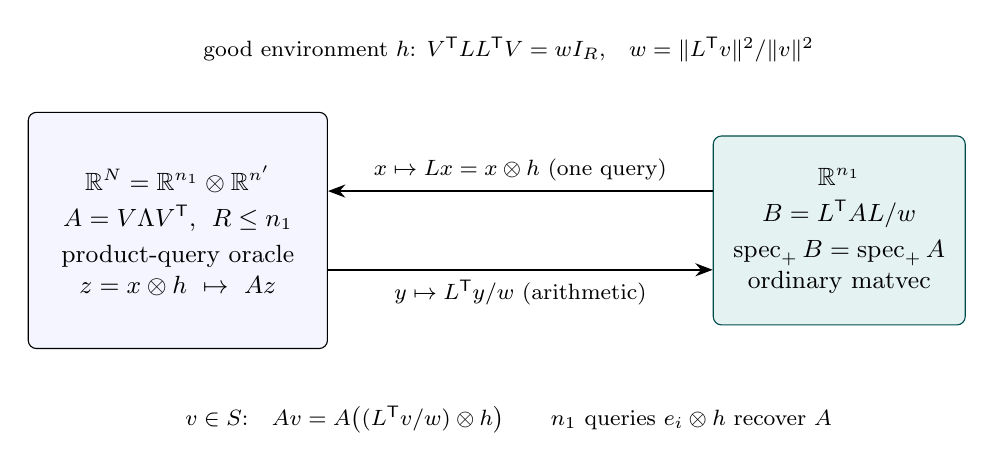
\begin{tikzpicture}[
  big/.style={draw,rounded corners=3pt,fill=blue!4,minimum width=38mm,
              minimum height=30mm,align=center,font=\small},
  small/.style={draw,rounded corners=3pt,fill=teal!10,draw=teal!60!black,
              minimum width=32mm,minimum height=24mm,align=center,font=\small},
  arr/.style={-{Stealth[length=2.2mm]},thick}]
\node[big] (A) at (0,0) {$\R^N=\R^{n_1}\otimes\R^{n'}$\\[2pt]
   $A=V\Lambda V^\T$, $\;R\le n_1$\\[2pt] product-query oracle\\
   $z=x\otimes h\ \mapsto\ Az$};
\node[small] (B) at (8.4,0) {$\R^{n_1}$\\[2pt] $B=L^\T AL/w$\\[2pt]
   $\operatorname{spec}_+B=\operatorname{spec}_+A$\\ ordinary matvec};
\draw[arr] ([yshift=5mm]B.west) -- node[above,font=\footnotesize]
   {$x\mapsto Lx=x\otimes h$ (one query)} ([yshift=5mm]A.east);
\draw[arr] ([yshift=-5mm]A.east) -- node[below,font=\footnotesize]
   {$y\mapsto L^\T y/w$ (arithmetic)} ([yshift=-5mm]B.west);
\node[font=\footnotesize,align=center] at (4.2,-2.4)
   {$v\in S$:\quad $Av=A\bigl((L^\T v/w)\otimes h\bigr)$\qquad
    $n_1$ queries $e_i\otimes h$ recover $A$};
\node[font=\footnotesize,align=center] at (4.2,2.3)
   {good environment $h$: $V^\T LL^\T V=wI_R$,\quad $w=\norm{L^\T v}^2/\norm v^2$};
\end{tikzpicture}
\caption{The $n_1$-dimensional reduction. One legal product query realizes one
product with the compressed matrix $B$, or one supported product with $A$.}
\label{fig:reduction}
\end{figure}

\begin{remark}[Exact arithmetic and conditioning]
All identities in this section are exact-arithmetic statements. A good but
unlucky environment may have small $w(h)$, which amplifies rounding error in
$L^\T v/w$. For two factors the environment $h_\star$ defined after
\eqref{eq:Srecover} has $w=1$; at higher order a random Gaussian
product environment, or the best of a few, is the practical choice.
No such identity is guaranteed for vectors outside $S$.
\end{remark}
\section{Generalized Nystr\"om}\label{sec:gn}

Generalized Nystr\"om \cite{TYUCgeneral,Nak} approximates a rectangular
$A\in\R^{N_L\times N_R}$ from a right sketch $Y=A\Omega$ ($k$ columns) and a
left sketch $X=\Psi^\T A$ ($p$ rows) by
\begin{equation}\label{eq:gn}
 \widehat A=Y(\Psi^\T Y)^\dagger X .
\end{equation}
By \eqref{eq:gn-q}, if $Q$ is an orthonormal basis of $\range Y$ and
$\Psi^\T Q$ has full column rank, then $\widehat A=Q(\Psi^\T Q)^\dagger\Psi^\T A$.
The left sketch therefore fixes a least-squares \emph{metric}, not only a
subspace, and this is where structured left sketches need care. Throughout,
$S_L=\range A$ with isometry $U\in\R^{N_L\times R}$, and the right and left
sketches are independent.

\begin{lemma}[Gaussian regression identity]\label{lem:regression}
Let $\range Y\subseteq S_L$ be $k$-dimensional with orthonormal basis $Q$, and
let $\widetilde\Psi\in\R^{N_L\times p}$, $p>k+1$, be independent of $Y$ with
$\widetilde\Psi^\T U$ having iid $N(0,1)$ entries. Then
$\widetilde A=Q(\widetilde\Psi^\T Q)^\dagger\widetilde\Psi^\T A$ satisfies
\begin{equation}\label{eq:regression}
 \E\bigl[\norm{A-\widetilde A}_\F^2\bigm| Q\bigr]
 =\Bigl(1+\frac k{p-k-1}\Bigr)\norm{(I-QQ^\T)A}_\F^2 .
\end{equation}
\end{lemma}

\begin{proof}
\emph{Step 1: split the Gaussian measurements into fitted and residual parts.}
Complete $Q$ to an orthonormal basis $[Q\ Q_\perp]$ of $S_L$. Conditionally on
$Q$, $\Gamma_1=\widetilde\Psi^\T Q$ and $\Gamma_2=\widetilde\Psi^\T Q_\perp$ are
independent standard Gaussian matrices, by rotation invariance. Since the
columns of $A$ lie in $S_L$, we have
\[
 \widetilde\Psi^\T A=\Gamma_1Q^\T A+\Gamma_2F,
 \qquad F=Q_\perp^\T A.
\]
Also $\Gamma_1^\dagger\Gamma_1=I_k$ almost surely.

\emph{Step 2: use orthogonality of the two error components.}
Writing $E=(I-QQ^\T)A=Q_\perp F$, we obtain
\[
 A-\widetilde A=E-Q\Gamma_1^\dagger\Gamma_2F.
\]
The two terms are Frobenius-orthogonal, and
\[
 \E\bigl[\norm{\Gamma_1^\dagger\Gamma_2F}_\F^2\mid\Gamma_1\bigr]
 =\norm{\Gamma_1^\dagger}_\F^2\norm F_\F^2.
\]
Lemma~\ref{lem:inverse} applied to $\Gamma_1^\T$ gives
$\E\norm{\Gamma_1^\dagger}_\F^2=k/(p-k-1)$, and $\norm F_\F=\norm E_\F$.
\end{proof}

\begin{theorem}[Structured right sketch, Gaussian left sketch]\label{thm:mixed}
Let the row space of $A$ satisfy Theorem~\ref{mthm:iff}, and let $\Psi$ be an
independent dense Gaussian matrix with $p>k+1$ columns. Then \eqref{eq:gn} has
exactly the output law of generalized Nystr\"om with Gaussian sketches on both
sides, and for $r+1<k$,
\begin{equation}\label{eq:gn-bound}
 \E\norm{A-\widehat A}_\F^2\le\Bigl(1+\frac k{p-k-1}\Bigr)
 \Bigl(1+\frac r{k-r-1}\Bigr)\tau_r^{(2)}(A).
\end{equation}
\end{theorem}

\begin{proof}
The output is range-determined (Lemma~\ref{lem:catalogue}(d)), so its law is
the Gaussian one. Lemma~\ref{lem:regression} with $\widetilde\Psi=\Psi$ and
Theorem~\ref{thm:rf} give \eqref{eq:gn-bound}; if $k\ge R$ the error is zero.
\end{proof}

The dense left sketch costs $p$ general left products, which may be
unavailable in a product-query model. The next two results make both sides
structured.

\subsection{Calibrated and frozen-environment reconstruction}

Let $S_L$ be in the conditionally Gaussian product class for a left generator,
and draw left probes $\psi_i=L_{\eta_i}g_i$, $i=1,\ldots,p$.

\emph{Calibrated estimator.} With independent environments $\eta_i$, choose a
nonzero column $v$ of $Y$ (it lies in $S_L$), compute
$w_i=\norm{L_{\eta_i}^\T v}^2/\norm v^2$ by \eqref{eq:calibration}, set
$D_L=\diag(\sqrt{w_1},\ldots,\sqrt{w_p})$, and return
\begin{equation}\label{eq:calGN}
 \widehat A_{\rm cal}=Y\bigl(D_L^{-1}\Psi^\T Y\bigr)^\dagger D_L^{-1}\Psi^\T A .
\end{equation}
The rescaling acts on stored rows and needs no further queries.

\emph{Frozen-environment estimator.} Draw one good environment $\eta_L$,
independent of everything else, and set $\psi_i=L_{\eta_L}g_i$. Return the
unmodified formula $\widehat A_{\rm fr}=Y(\Psi^\T Y)^\dagger\Psi^\T A$.

\begin{theorem}[Structured generalized Nystr\"om]\label{thm:calGN}
In both constructions, conditionally on $Q$,
\begin{equation}\label{eq:calGN-id}
 \E\bigl[\norm{A-\widehat A}_\F^2\bigm| Q\bigr]
 =\Bigl(1+\frac k{p-k-1}\Bigr)\norm{(I-QQ^\T)A}_\F^2 ,
\end{equation}
for any independent right sketch with $\rank Y=k$. If in addition the row
space of $A$ satisfies Theorem~\ref{mthm:iff} (for instance, it is in the
conditionally Gaussian product class for the right generator, with
independent or frozen right environments), then $\widehat A_{\rm cal}$ and
$\widehat A_{\rm fr}$ both have exactly the two-Gaussian output law and satisfy
\eqref{eq:gn-bound}.
\end{theorem}

\begin{proof}
\emph{Calibrated case.} By Theorem~\ref{thm:calibration}, $\widetilde\Psi=\Psi D_L^{-1}$
has $\widetilde\Psi^\T U$ iid Gaussian, independent of the environments and of
the right sketch (the weights are the exact values $w(\eta_i)$, whichever
supported $v$ is used). Moreover
\[
 \widehat A_{\rm cal}
 =Y(\widetilde\Psi^\T Y)^\dagger\widetilde\Psi^\T A
 =Q(\widetilde\Psi^\T Q)^\dagger\widetilde\Psi^\T A.
\]

\emph{Frozen case.} Conditionally
on $\eta_L$, $\Psi^\T U=\sqrt{w(\eta_L)}\,\Gamma$ with $\Gamma$ standard Gaussian,
and a common positive scalar cancels,
$(c\,\Psi^\T Q)^\dagger c\,\Psi^\T A=(\Psi^\T Q)^\dagger\Psi^\T A$; so
$\widehat A_{\rm fr}=Q(\widetilde\Psi^\T Q)^\dagger\widetilde\Psi^\T A$ with
$\widetilde\Psi=\Psi/\sqrt{w(\eta_L)}$, and the conditional law of
$\widetilde\Psi^\T U$ does not depend on $\eta_L$.

\emph{Combine the two independent Gaussian ingredients.} In both cases
Lemma~\ref{lem:regression} gives \eqref{eq:calGN-id}. Each output is a
measurable function of $\range Y$ and $\widetilde\Psi^\T U$, since
$\widetilde\Psi^\T A=\widetilde\Psi^\T UU^\T A$ and $Q\subseteq S_L$. Under the
right-side hypothesis, $\range Y$ has the Gaussian law
(Theorem~\ref{mthm:iff}, Remark~\ref{rem:frozen-range}) and is independent of
$\widetilde\Psi^\T U$, which is standard Gaussian: this is exactly the joint law
in two-sided Gaussian generalized Nystr\"om. The bound follows from
Theorem~\ref{thm:rf}.
\end{proof}

\begin{corollary}[A $6r+8$ product-query budget]\label{cor:6r8}
Under the hypotheses of Theorem~\ref{thm:calGN} with the right-side condition,
$k=2r+2$ and $p=2k+2$ use $k+p=6r+8$ product queries and give
\[
 \E\norm{A-\widehat A}_\F^2\le\frac{(4r+5)(2r+1)}{(2r+3)(r+1)}\,\tau_r^{(2)}(A)
 \le4\,\tau_r^{(2)}(A),
\]
with no truncation step, for both $\widehat A_{\rm cal}$ and $\widehat A_{\rm fr}$.
The rational prefactor is strictly below four; the last inequality is strict
when $\tau_r^{(2)}(A)>0$.
The frozen-environment version needs no calibration weights at all. If
$\rank A\le k$ and $p\ge\rank A$, the reconstruction is exact almost surely.
\end{corollary}

\begin{proof}
$1+\frac{k}{p-k-1}=\frac{4r+5}{2r+3}<2$ and $1+\frac r{k-r-1}=\frac{2r+1}{r+1}<2$.
\end{proof}

By Markov's inequality the squared-error factor is at most $20$ with
probability at least $4/5$. All query vectors of both constructions can be
drawn before any response is observed; only the calibration weights use a
response. The frozen design changes the \emph{sampling law} (the environment
is shared within the left sketch); it is not a statement about the original
independently regenerated Khatri--Rao columns, for which see
Proposition~\ref{prop:raw}.
\subsection{The raw estimator with independent left environments}

With independent left environments and no calibration, the column scales
multiply the left measurements \emph{on the left}, and they do not cancel from
least squares (Proposition~\ref{prop:leftscaling} below). A bound still holds,
through a weighted inverse.

\begin{lemma}[Size-biased monotonicity]\label{lem:monotone}
If $w>0$, $\E w=1$, $\E w^2<\infty$, and $f\ge0$ is nonincreasing, then
$\E[w^2f(w)]\le(\E w^2)\,\E[wf(w)]$.
\end{lemma}

\begin{proof}
Under $d\mathbb Q=w\,d\Prob$, the increasing function $w$ and the nonincreasing
$f(w)$ have nonpositive covariance (average $(w-w')(f(w)-f(w'))\le0$ over two
independent copies). Since $\E_{\mathbb Q}[wf(w)]=\E[w^2f(w)]$,
$\E_{\mathbb Q}w=\E w^2$ and $\E_{\mathbb Q}f(w)=\E[wf(w)]$, the claim follows.
\end{proof}

\begin{proposition}[Raw two-structured-sketch reconstruction]\label{prop:raw}
Let $q=2$ on the left, let $S_L$ satisfy Proposition~\ref{prop:test} with
matrix $S_0$, and use iid left probes $\psi_i=g_i\otimes h_i$. Put
$\mu_2=\E(h^\T S_0h)^2=1+2\tr S_0^2\le3$. For $p\ge4(k+1)$, the raw estimator
$\widehat A_{\rm raw}=Y(\Psi^\T Y)^\dagger\Psi^\T A$ satisfies
\[
 \E\bigl[\norm{A-\widehat A_{\rm raw}}_\F^2\bigm| Q\bigr]
 \le\Bigl(1+\mu_2C_{\rm new}\frac kp\Bigr)\norm{(I-QQ^\T)A}_\F^2,
 \qquad C_{\rm new}=\frac{112}{3\pi}-\frac43 .
\]
\end{proposition}

\begin{proof}
\emph{Step 1: write the weighted regression error.}
With the notation of Lemma~\ref{lem:regression}, the left coordinates are
$\Psi^\T Q=W^{1/2}\Xi$ and $\Psi^\T Q_\perp=W^{1/2}\Xi'$, where
$W=\diag(w_i)$, $w_i=h_i^\T S_0h_i$, and $\Xi,\Xi'$ are independent standard
Gaussian and independent of $W$ (Theorem~\ref{thm:mechanism}). With
$H=\Xi^\T W\Xi$, the pseudoinverse is
$(W^{1/2}\Xi)^\dagger=H^{-1}\Xi^\T W^{1/2}$ and
\[
 A-\widehat A_{\rm raw}=E-QH^{-1}\Xi^\T W\Xi'F.
\]
Averaging over $\Xi'$ gives the conditional error
$(1+\mathcal B)\norm E_\F^2$, where
\[
 \mathcal B=\E\tr(H^{-1}\Xi^\T W^2\Xi H^{-1})
 =\E\sum_iw_i^2\xi_i^\T H^{-2}\xi_i,
\]
where $\xi_i^\T$ are the rows of $\Xi$. For $\eta>0$ and fixed other variables,
$f_i(w_i)=\xi_i^\T(H+\eta I)^{-2}\xi_i$ is nonincreasing in $w_i$, since
\[
 f_i'=-2\bigl(\xi_i^\T(H+\eta I)^{-1}\xi_i\bigr)f_i\le0.
\]

\emph{Step 2: remove one weight by size-biased monotonicity.}
Since $w_i$ is independent of
the rest and $\E w_i=\tr S_0=1$, Lemma~\ref{lem:monotone} and summation give
\[
 \begin{aligned}
 \E\tr\bigl((H+\eta I)^{-1}\Xi^\T W^2\Xi(H+\eta I)^{-1}\bigr)
 &\le\mu_2\E\tr\bigl(H(H+\eta I)^{-2}\bigr)\\
 &\le\mu_2\E\tr H^{-1}.
 \end{aligned}
\]
Let $\eta\downarrow0$ by monotone convergence.

\emph{Step 3: apply the weighted inverse bound.} By rotation
invariance of $h$, $w$ has the law of $\sum_b\lambda_b(S_0)h_b^2$, which is the
common-Schmidt weight law, so Theorem~\ref{imp:kr} (at dimension $k$,
sample size $p$) gives $\E\tr H^{-1}=p^{-1}\E\tr S_p^{-1}\le C_{\rm new}k/p$.
Finally $\E w^2=(\tr S_0)^2+2\tr S_0^2$.
\end{proof}

With $\mu_2\le3$, $3C_{\rm new}<31.651$, so $k=2r+2$ and $p=32k$ give an expected
squared-error factor below four, using $66r+66$ product queries, against
$6r+8$ for the calibrated and frozen versions. The comparison reflects the
constant in the weighted inverse bound more than a real gap: in simulations
the coefficient $\mathcal B$ is about $9$--$11$ times smaller than $\mu_2C_{\rm new}k/p$
(Section~\ref{sec:numerics}).

\subsection{Two unnormalized structured sides}

If the left support also satisfies the mechanism, then
$U^\T\Psi=\Gamma E_0$ with a random positive diagonal $E_0$, so the left
measurements are multiplied on the left by $E_0$. In overdetermined least
squares $(E_0M)^\dagger E_0\ne M^\dagger$ in general.

\begin{proposition}[Left scaling changes generalized Nystr\"om]
\label{prop:leftscaling}
Let $A=I_2$, $Y=e_1$, $\Psi^\T=\bigl[\begin{smallmatrix}1&1\\1&-1\end{smallmatrix}\bigr]$
and $E_0=\diag(1,t)$, $t>0$. The unweighted estimate
$Y(\Psi^\T Y)^\dagger\Psi^\T A$ equals $e_1[1\ \ 0]$, with squared error $1$. With
the rescaled left sketch $\Psi E_0$ it equals
\[
 e_1\Bigl[1\ \ \ \tfrac{1-t^2}{1+t^2}\Bigr],\qquad\text{with squared error }
 1+\Bigl(\tfrac{1-t^2}{1+t^2}\Bigr)^2 .
\]
Both left sketches have the same column span.
\end{proposition}

\begin{proof}
$\Psi^\T Y=(1,1)^\T$ has pseudoinverse $\frac12(1,1)$, and
$\frac12(1,1)\Psi^\T=(1,0)$. With $E_0$: $E_0\Psi^\T Y=(1,t)^\T$ has pseudoinverse
$(1,t)/(1+t^2)$, and $(1,t)E_0\Psi^\T/(1+t^2)=(1+t^2,1-t^2)/(1+t^2)$. The error
matrix is $\bigl[\begin{smallmatrix}0&-c\\0&1\end{smallmatrix}\bigr]$ with
$c=(1-t^2)/(1+t^2)$.
\end{proof}

So column-span equivalence alone cannot give the two-sided estimator a Gaussian
law; the example refutes that invariance, not the existence of good structured
algorithms. The remedies are exactly the constructions of
Theorem~\ref{thm:calGN}: rescale by the known weights (calibration,
equivalently $\Psi\mapsto\Psi E_0^{-1}$), or make the left scale common to all
columns (frozen environment), which then cancels.

\begin{remark}[Relation to an open question on general inputs]
Cama\~no, Epperly, Meyer and Tropp \cite[Remark~2.9]{CEMT} analyse
generalized Nystr\"om with structured sketches through oblivious subspace
injections, with $k=\gamma r$ right and $p=\gamma^2r$ left columns for an
oversampling factor $\gamma$, and ask whether $p=O(\gamma r)$ suffices without
truncation. On the class studied here both stages are Gaussian-equivalent,
$\gamma=O(1)$, and the question does not arise. It concerns general inputs,
where neither the support structure nor the left calibration is available.
One concrete bridge would be a bound
$\E_\Psi\norm{(\Psi^\T Q)^\dagger\Psi^\T E}_\F^2\le C\norm E_\F^2$ for
$Q^\T E=0$ and economical structured $\Psi$; Lemma~\ref{lem:regression} is its
Gaussian case.
\end{remark}
\section{Calibrated trace estimation}\label{sec:trace}

The estimator combines a Nystr\"om approximation with a calibrated Hutchinson
correction, as in Nystr\"om++ \cite{Nyspp} and Hutch++ \cite{Hutchpp}. We
first prove the Gaussian Nystr\"om residual bound it needs, by a drift
argument; the same argument with a product-dependent constant governs
unrestricted inputs in ``Product-Probe Drift, Kronecker Nystr\"om
Approximation, and Trace Estimation'' \cite{PPD}.

\begin{lemma}[Residual update]\label{lem:update}
Let $A\succeq0$, let $C_t$ be the Nystr\"om approximation from test vectors
$z_1,\ldots,z_t$ and $R_t=A-C_t$. If $z_{t+1}^\T R_tz_{t+1}>0$ then
$R_{t+1}=R_t-R_tz_{t+1}z_{t+1}^\T R_t/(z_{t+1}^\T R_tz_{t+1})$; otherwise
$R_{t+1}=R_t$. In particular $0\preceq R_{t+1}\preceq R_t$.
\end{lemma}

\begin{proof}
By \eqref{eq:nys-projector}, $R_t=A^{1/2}(I-P_t)A^{1/2}$ with $P_t$ the projector
onto $\range(A^{1/2}Z_t)$. Adding $z=z_{t+1}$ adds to $P_t$ the rank-one
projector onto $x=(I-P_t)A^{1/2}z$ when $x\ne0$, and
$A^{1/2}xx^\T A^{1/2}/\norm x^2=R_tzz^\T R_t/(z^\T R_tz)$.
\end{proof}

\begin{lemma}[Gaussian drift]\label{lem:drift}
Let $R\succeq0$, $R\ne0$, and $g\sim N(0,I)$. Then
\[
 \E\frac{g^\T R^2g}{g^\T Rg}\ \ge\ \frac{\tr R^2}{\kapG\tr R},\qquad
 \kapG=\exp(2-\gamma-\log2)=\frac{e^{2-\gamma}}2=2.0743278\ldots
\]
\end{lemma}

\begin{proof}
\emph{Step 1: tilt by the numerator.}
Let $X=g^\T Rg$, $Y=g^\T R^2g$, and
$d\mathbb Q=(Y/\tr R^2)\,d\Prob$. Jensen's inequality gives
\[
 \E[Y/X]=\tr R^2\,\E_{\mathbb Q}[X^{-1}]
 \ge\tr R^2\exp(-\E_{\mathbb Q}\log X).
\]
For $\beta\in(0,1)$, a second use of Jensen yields
\[
 \E_{\mathbb Q}\log X\le\beta^{-1}\log\E_{\mathbb Q}X^\beta.
\]
The Gaussian gamma integrals below also ensure the required logarithmic
integrability.

\emph{Step 2: bound the tilted fractional moment.} Diagonalize
$R=\sum_i\mu_iu_iu_i^\T$ and put $z_i=(u_i^\T g)^2$, iid $\chi^2_1$ with
$\E z_i^p=c(p):=2^p\Gamma(p+\frac12)/\sqrt\pi$. By H\"older with exponents
$1+\beta$ and $(1+\beta)/\beta$, and Minkowski in $L^{1+\beta}$,
\[
 \begin{aligned}
 \E[z_iX^\beta]
 &\le c(1+\beta)^{\frac1{1+\beta}}
       \bigl(\E X^{1+\beta}\bigr)^{\frac\beta{1+\beta}}\\
 &\le c(1+\beta)^{\frac1{1+\beta}}
       \bigl(c(1+\beta)^{\frac1{1+\beta}}\tr R\bigr)^\beta\\
 &=c(1+\beta)(\tr R)^\beta .
 \end{aligned}
\]
Consequently,
\[
 \E_{\mathbb Q}X^\beta
 =\frac{\sum_i\mu_i^2\E[z_iX^\beta]}{\tr R^2}
 \le c(1+\beta)(\tr R)^\beta.
\]

\emph{Step 3: let the moment order tend to one.}
Substituting in Step 1 gives
\[
 \E[Y/X]\ge\frac{\tr R^2}{c(1+\beta)^{1/\beta}\tr R}.
\]
As $\beta\downarrow0$,
\[
 c(1+\beta)^{1/\beta}
 \longrightarrow\exp\!\left(\left.\frac{d}{dp}\log c(p)\right|_{p=1}\right)
 =\exp\bigl(\log2+\psi(\tfrac32)\bigr)=\kapG,
\]
where $\psi(\frac32)=2-\gamma-2\log2$.
\end{proof}

\begin{lemma}[Nystr\"om residual]\label{lem:residual}
If $A\succeq0$ has range $S$ satisfying Theorem~\ref{mthm:iff}, and $C$ is the
Nystr\"om approximation from $m$ probes, then
$\E\norm{A-C}_\F^2\le\kapG(\tr A)^2/m$.
\end{lemma}

\begin{proof}
$\norm{A-C}_\F^2$ is a function of $C$, which is range-determined, so we may
use Gaussian probes. The case $A=0$ is immediate, so put $T=\tr A>0$.
By Lemmas~\ref{lem:update}
and~\ref{lem:drift} (applied to $V^\T R_tV$ and $V^\T z_{t+1}\sim N(0,I_R)$,
independent of $R_t$),
\[
 \E[\tr R_t-\tr R_{t+1}\mid R_t]
 \ge\frac{\tr R_t^2}{\kapG\tr R_t},
\]
with $0/0=0$. The trace loss telescopes, so
\[
 \sum_{t<m}\E\frac{\tr R_t^2}{\tr R_t}\le\kapG T.
\]
Since
$\tr R_t\le T$ and $\tr R_t^2\ge\tr R_m^2$ (as $0\preceq R_m\preceq R_t$), each
term is at least $\E\tr R_m^2/T$. Thus
$m\E\norm{R_m}_\F^2/T\le\kapG T$, as required.
\end{proof}

\paragraph{The estimator.} Let $A\succeq0$ have range $S$ in the conditionally
Gaussian product class. Given $\eps\in(0,1)$, put
$m=s=\lceil\sqrt{6\kapG}/\eps\rceil$.
\begin{itemize}
\item If $2m\ge n_1$: draw a random good environment $h$, query $A(e_i\otimes h)$
      for $i\le n_1$, read $w$ from a nonzero response, and return
      $\widehat T=\tr(L_h^\T AL_h)/w$ (return $0$ if all responses vanish).
\item Otherwise: draw $m$ independent Gaussian product probes $Z$, form $Y=AZ$
      and $C=Y(Z^\T Y)^\dagger Y^\T$, take a nonzero column $v$ of $Y$ (if none,
      return $0$), draw $s$ independent test probes $\omega_j=L_{\eta_j}g_j$,
      compute $w_j=\norm{L_{\eta_j}^\T v}^2/\norm v^2$, and return
      \begin{equation}\label{eq:traceest}
       \widehat T=\tr C+\frac1s\sum_{j=1}^s\frac{\omega_j^\T(A\omega_j-C\omega_j)}{w_j}.
      \end{equation}
\end{itemize}
All query vectors are chosen before any response is seen, and every query is a
legal product; $C\omega_j$ is computed by arithmetic.

\begin{proof}[Proof of Theorem~\ref{mthm:trace}]
The first branch uses $n_1$ queries and is exact by
Theorem~\ref{mthm:reduction}(d). In the second branch, $2m<n_1$ queries are
used. Let $\widetilde R=V^\T(A-C)V$ and $g_j=V^\T\omega_j/\sqrt{w_j}$. The range of
$A-C$ lies in $S$, so $\omega_j^\T(A-C)\omega_j/w_j=g_j^\T\widetilde Rg_j$. By
Theorem~\ref{thm:calibration}, the $g_j$ are iid $N(0,I_R)$ and independent of
$Z$ and hence of $C$. Therefore $\E[\widehat T\mid C]=\tr C+\tr\widetilde R=T$ and
$\Var(\widehat T\mid C)=2\norm{A-C}_\F^2/s$. By Lemma~\ref{lem:residual},
\[
 \Var\widehat T=\E\Var(\widehat T\mid C)\le\frac{2\kapG}{ms}T^2,
\]
and Chebyshev's inequality with $ms\ge6\kapG/\eps^2$ gives failure probability
at most $1/3$. If $m\ge R$, the lines $[V^\T z_i]$ are iid uniform and span
$\R^R$ almost surely, so $C=A$ and $\widehat T=T$.
\end{proof}

The leading constant is $2\sqrt{6\kapG}=7.0557684$, so the count is
$\min\{7.06/\eps+2,\,n_1\}$ up to rounding. A median of $O(\log(1/\delta))$
independent repetitions gives confidence $1-\delta$ (the median need not be
unbiased), and all queries can still be fixed in advance.

\begin{remark}[What the theorem is]
After calibration, the approximation and test probes project to iid Gaussian
vectors on $S$, so the second branch has exactly the law of Gaussian
Nystr\"om++ on the $R$-dimensional support, equivalently on the compressed
matrix $B$ of Theorem~\ref{mthm:reduction}. The $O(1/\eps)$ rate is therefore the
familiar Gaussian rate \cite{Hutchpp,Nyspp}, realized with product queries, and
not a new trace-estimation principle. It is informative only when $n_1$ (and
$\rank A$) is much larger than about $7/\eps$; otherwise $n_1$ product queries
give the trace exactly. The cap uses $n_1$, which is known in advance, rather
than the unknown $\rank A$. For general PSD inputs, product-query trace
estimation is a different and harder problem; see the product-probe companion \cite{PPD} and the general-input lower bounds of \cite{MSW}.
\end{remark}
\section{Where the equivalence stops}\label{sec:limits}

\subsection{A Gaussian range law is not a Gaussian embedding law}

Take $u=e_1\otimes f$ with $f$ a unit vector, and the Gaussian Khatri--Rao
probe $\omega=g\otimes h$. The projected coordinate is
$\langle u,\omega\rangle=g_1\langle f,h\rangle$, a product of two independent
standard Gaussians: its second moment is $1$ and its fourth moment is $9$,
against $3$ for a Gaussian. One nonzero probe already spans this
one-dimensional support, so every range-determined output is exact and has the
Gaussian law, while the sketch Gram law is not Gaussian. In general, under
\eqref{eq:GD},
\[
 (V^\T\Omega)(V^\T\Omega)^\T=GD^2G^\T,
\]
and $D$ cannot be discarded. Embedding distortion, inverse-Gram moments and
numerical conditioning are different observables. Nothing here supersedes
Khatri--Rao embedding results \cite{BM,SVB,BGKL} or oblivious subspace injection
bounds \cite{CEMT}.

\subsection{A hypothesis on the leading eigenvectors alone is insufficient}

Let $n_1=n_2=2$, $u_1=e_1\otimes e_1$, $u_2=e_2\otimes e_2$, and
$A=\mu_1u_1u_1^\T+\mu_2u_2u_2^\T$ with $\mu_1\ge\mu_2>0$. Each $u_a$ separately
has the common-Schmidt form, and the leading eigenvector $u_1$ alone meets the
mechanism. The support $S=\operatorname{span}\{u_1,u_2\}$ does not: the
projected probe $(g_1h_1,g_2h_2)$ has conditional covariance
$\diag(h_1^2,h_2^2)$, and its line is not uniform. The effect on the output is
explicit.

\begin{proposition}[Head-only counterexample]\label{prop:headonly}
Let $C$ be the one-column Nystr\"om approximation of $A$ and $y=\sqrt{\mu_2/\mu_1}\in(0,1]$.
For a dense Gaussian probe $\E\tr(A-C)=\sqrt{\mu_1\mu_2}$. For the Gaussian
Khatri--Rao probe
\[
 \E\tr(A-C)=\sqrt{\mu_1\mu_2}\;\Phi(y),\qquad
 \Phi(y)=\frac{2y+\frac2\pi(1-y^2)\log(1/y)}{1+y^2}.
\]
$\Phi(1)=1$, $\Phi(y)>1$ for $0<y<1$, and $\Phi(y)\sim\frac2\pi\log(1/y)$ as
$y\to0$. Even at $y=1$, where the trace error is the constant $\mu_1$ for both
probes, the output laws differ: $\range C$ is the line of slope $c$ spanned by
the projected probe, and $\log|c|$ has variance $\pi^2/2$, against $\pi^2/4$
for the Gaussian.
\end{proposition}

\begin{proof}
\emph{Step 1: express the error through the projected slope.}
For a probe with projected coordinates $(c_1,c_2)$ and $c=c_2/c_1$,
\[
 \tr(A-C)=\frac{\mu_1\mu_2(c_1^2+c_2^2)}{\mu_1c_1^2+\mu_2c_2^2}
 =\frac{\mu_1\mu_2(1+c^2)}{\mu_1+\mu_2c^2}.
\]
Normalize $\mu_1=1$, $\mu_2=y^2$. The ratio of the mean error to
$\sqrt{\mu_1\mu_2}=y$ is $\E\,y(1+c^2)/(1+y^2c^2)$. The decomposition
\[
 \frac{1+c^2}{1+y^2c^2}
 =y^{-2}+\frac{1-y^{-2}}{1+y^2c^2}
\]
reduces the calculation to one Cauchy integral.

\emph{Step 2: average the random Cauchy scale.} If $c$ is Cauchy with scale
$a$, convolution of Cauchy kernels gives $\E[1/(1+y^2c^2)]=1/(1+ay)$.
For a Gaussian probe, $c$ is standard Cauchy ($a=1$), and the ratio equals
$y[y^{-2}+(1-y^{-2})/(1+y)]=1$. For a Khatri--Rao probe,
$c=(g_2/g_1)(h_2/h_1)$ is Cauchy with random scale $a=|h_2/h_1|$, whose density
is $2/(\pi(1+a^2))$ on $a>0$, and a partial-fraction computation gives
\[
 \E_a\frac1{1+ay}=\frac2\pi\int_0^\infty\frac{da}{(1+a^2)(1+ay)}
 =\frac{1+\frac2\pi y\log y}{1+y^2}.
\]
Substitution yields the stated expression for $\Phi$.

\emph{Step 3: show the gap and distinguish the equal-eigenvalue laws.}
We have
\[
 \Phi(y)-1
 =\frac{(1-y)[\frac2\pi(1+y)\log(1/y)-(1-y)]}{1+y^2}.
\]
The inequality
$\log(1/y)\ge2(1-y)/(1+y)$ gives
$\frac2\pi(1+y)\log(1/y)\ge\frac4\pi(1-y)>1-y$ for $y<1$. Finally
$\log|c|$ is a sum of two independent copies of $\log|g_2/g_1|$, each of
variance $2\cdot\pi^2/8=\pi^2/4$, against one copy for the Gaussian.
\end{proof}

The requirement is on the \emph{entire} relevant support, spectral tail
included. A certificate for the leading $r$ eigenvectors says nothing about
the joint law of the head and tail coordinates on which the error bounds rest.

\subsection{Weight-sensitive surrogates do not cancel}

Deterministic bounds are often proved with the candidate coefficient matrix
$(G_1D)^\dagger$, which produces the surrogate $G_2D(G_1D)^\dagger$. The
weights do not cancel from it. The range also admits the coefficient
$D^{-1}G_1^\dagger$, which produces $G_2G_1^\dagger$, and the second is never worse.

\begin{proposition}[Surrogate domination]\label{prop:surrogate}
Let $G_1\in\R^{r\times k}$ have full row rank, $D$ be invertible diagonal, and
$G_2$ be an independent standard Gaussian matrix. For every $\Lambda_2\succeq0$,
\[
 \begin{aligned}
 \E_{G_2}\norm{\Lambda_2^{1/2}G_2D(G_1D)^\dagger}_\F^2
 &=\tr\Lambda_2\,\norm{D(G_1D)^\dagger}_\F^2\\
 &\ge\tr\Lambda_2\,\norm{G_1^\dagger}_\F^2\\
 &=\E_{G_2}\norm{\Lambda_2^{1/2}G_2G_1^\dagger}_\F^2 .
 \end{aligned}
\]
\end{proposition}

\begin{proof}
The equalities are Gaussian second moments. $D(G_1D)^\dagger$ is a right inverse of
$G_1$, since $G_1D(G_1D)^\dagger=I_r$, and $G_1^\dagger$ is the right inverse of
minimal Frobenius norm.
\end{proof}

This is the reason the weighted inverse route in
Theorem~\ref{imp:kr} yields a coefficient about $31.65\,r/k$ whereas the exact
range law yields $r/(k-r-1)$. There is no conflict: the first is one valid
candidate bound, while the approximation depends on the whole range.

\subsection{Two unnormalized structured sides; exact arithmetic}

Proposition~\ref{prop:leftscaling} shows that independent left scales change
generalized Nystr\"om even when the left span is unchanged, so the two-sided
estimator with independently regenerated structured sketches on both sides
has no automatic Gaussian law; Proposition~\ref{prop:raw} bounds it with a
worse constant. Finally, all statements concern exact projectors and
pseudoinverses. Very small column scales can make a floating-point
implementation discard a column or misjudge a rank; column equilibration may
help but needs its own numerical analysis.
\section{Numerical illustrations}\label{sec:numerics}

All experiments below are numerical checks of proved statements, run in
Julia~1.13 in double precision with fixed seeds. They are diagnostics, not
proofs. ``Common-Schmidt'' supports are generated from random orthonormal
$e_{a,b}$ and $f_b$ as in \eqref{eq:schmidt}. The six Julia scripts and their
rerun outputs are included in the
\href{https://github.com/DiarHaidary/Results/tree/main/manuscripts/03-Exact-Gaussian-Range-Laws/checks}{repository checks directory}.
An independent Python audit also checks the added weighted-inverse constant
over $10{,}000$ admissible budgets, the radial distribution-function bound,
the closed-form counterexample, and the matrix identities. These finite
checks supplement the proofs and do not certify floating-point stability.

\paragraph{Exact laws.} Table~\ref{tab:laws} compares Gaussian Khatri--Rao
Nystr\"om with dense Gaussian Nystr\"om on a common-Schmidt input
($n_1=12$, $n_2=3$, $\ell=2$, weights $(0.7,0.3)$, $R=6$, eigenvalues
$10,5,1,0.5,0.3,0.2$, $r=2$, $k=4$, $20{,}000$ trials). Means and quantiles
agree within Monte Carlo error, and both sit well below the bound
$(1+r/(k-r-1))\tau_r=6$ of Corollary~\ref{cor:kr}.

\begin{table}[htbp]
\centering\small
\begin{tabular}{@{}lccccc@{}}\toprule
& mean $\tr(A-C)$ & mean $\tr(A-C_r)$ & 10\% & 50\% & 90\%\\\midrule
Khatri--Rao & 1.7007 & 2.8526 & 2.1246 & 2.5284 & 3.9731\\
Gaussian    & 1.6933 & 2.8431 & 2.1241 & 2.5303 & 3.9734\\\bottomrule
\end{tabular}
\caption{Common-Schmidt Khatri--Rao versus Gaussian Nystr\"om; quantiles are of
$\tr(A-C_r)$.}
\label{tab:laws}
\end{table}

Further law checks:
\begin{itemize}
\item \emph{Hurwitz pair} (Example~\ref{ex:hurwitz}): the identities hold to
      $1.6\times10^{-16}$; the angle of $V^\T\omega$ in eight bins of width
$\pi/8$ on $[0,\pi)$ has frequencies $0.124$--$0.126$ (uniform: $0.125$), $2\times10^5$
      samples.
\item \emph{Spherical factors} (Corollary~\ref{cor:spherical}; $R=3$): the
      direction of $V^\T\omega$ has $\norm{\E uu^\T-I/3}=0.0020$ and
      $\E u_1^4=0.1990$ against $0.2$ for the uniform law on $S^2$.
\item \emph{Single-core tensor train} (Proposition~\ref{prop:tt}; $q=3$,
      $\chi=2$): $\E\norm\omega^2/N=1.002$, and the direction histogram is
      uniform within $0.003$. The fourth moment of one projected coordinate
      over its squared variance is $13.4$, against $3$ for a Gaussian: the range
      law is Gaussian, the embedding law is not.
\item \emph{Head-only counterexample} (Proposition~\ref{prop:headonly}):
      Table~\ref{tab:headonly}; $2\times10^6$ samples per row. The variance of the
      log absolute slope is $4.9255$ for Khatri--Rao ($\pi^2/2=4.9348$) and
      $2.4674$ for Gaussian ($\pi^2/4=2.4674$). A quadrature of $\Phi$ against the
      product-of-Cauchy density agrees with the closed form to six digits.
\end{itemize}

\begin{table}[htbp]
\centering\small
\begin{tabular}{@{}cccccc@{}}\toprule
$(\mu_1,\mu_2)$ & Gaussian MC & $\sqrt{\mu_1\mu_2}$ & Khatri--Rao MC &
$\sqrt{\mu_1\mu_2}\Phi(y)$ & $\Phi(y)$\\\midrule
$(1,0.25)$   & 0.4997 & 0.5000 & 0.5327 & 0.5324 & 1.065\\
$(1,0.01)$   & 0.1000 & 0.1000 & 0.1634 & 0.1635 & 1.635\\
$(1,10^{-4})$& 0.0101 & 0.0100 & 0.0295 & 0.0295 & 2.951\\\bottomrule
\end{tabular}
\caption{One-column Nystr\"om trace error in the head-only counterexample.}
\label{tab:headonly}
\end{table}

\paragraph{Dimension counts.} For the Segre cone with $(n_j)=(2,2)$, $(2,2,2)$,
$(2,2,2,2,2)$, $(3,4)$ and $(3,3,3)$, the generic Jacobian rank of
$(x_j)\mapsto x_1\otimes\cdots\otimes x_q$ equals $\delta+1$ in every case. The
generic rank of the differential of the map from $k$ product probes to
$\range(V^\T\Omega)\in\Gr(k,R)$, for a random $R$-dimensional $V$, is
$\min\{k\delta,k(R-k)\}$ in all tested cases (Table~\ref{tab:grass}), so the
bound $R\le k+\delta$ of Theorem~\ref{mthm:ceiling}(ii) is exactly the point where
the image stops being full-dimensional. The hook probe of
Example~\ref{ex:hook} with $(n_j)=(3,2,4)$ reproduces
$V^\T\omega=(z_0,z_1,\ldots,z_q)$ to $1.9\times10^{-16}$ on a support of dimension
$\delta+1=7$.

\begin{table}[htbp]
\centering\small
\begin{tabular}{@{}ccccccc@{}}\toprule
$(n_j)$ & $k$ & $R$ & image dim & $k\delta$ & $k(R-k)$ & $R\le k+\delta$\\\midrule
$(2,2,2)$ & 1 & 4 & 3 & 3 & 3 & yes\\
$(2,2,2)$ & 1 & 5 & 3 & 3 & 4 & no\\
$(2,2,2)$ & 2 & 5 & 6 & 6 & 6 & yes\\
$(2,2,2)$ & 2 & 6 & 6 & 6 & 8 & no\\
$(2,2,2)$ & 3 & 7 & 9 & 9 & 12 & no\\
$(2,2,2)$ & 4 & 8 & 12 & 12 & 16 & no\\
$(3,3)$   & 2 & 6 & 8 & 8 & 8 & yes\\
$(3,3)$   & 2 & 7 & 8 & 8 & 10 & no\\\bottomrule
\end{tabular}
\caption{Generic dimension of the image of product-probe ranges in $\Gr(k,R)$.}
\label{tab:grass}
\end{table}
\paragraph{The $n_1$-dimensional reduction.} On a two-factor common-Schmidt
input ($n_1=12$, $n_2=4$, weights $(0.6,0.3,0.1)$, $R=4$, eigenvalues
$10,3,1,0.2$) with a random frozen environment:
$\norm{V^\T LL^\T V-wI}=4.9\times10^{-16}$; the one-query product
$A((L^\T v/w)\otimes h)$ matches $Av$ to relative error $1.6\times10^{-16}$, and
$w$ read from a response matches to $1.5\times10^{-16}$; for an unsupported $v$
the error is $2.95$, as it must be. The compressed matrix has spectrum
$(10,3,1,0.2,0,\ldots)$; Nystr\"om from the $n_1=12$ queries $e_i\otimes h$
recovers $A$ to $4.7\times10^{-16}$ with $\tr B=\tr A$; five powers computed with
one query each match to $7.5\times10^{-16}$. At third order ($n=(6,2,2)$, entangled
$f_b$), over $1000$ random frozen product environments the worst relative
error of the one-query identity is $4.8\times10^{-15}$. For a rectangular input,
four cycles of $AA^\T$ with two queries each match to $4.1\times10^{-16}$; the
compressed matrix has singular values $(5,3,2,1,0.5,0,\ldots)$; exact recovery
from $n_1$ right and $n_1$ left product queries has error $5.4\times10^{-16}$; the
log-determinant identity of Corollary~\ref{cor:spectral} holds to rounding, and
a lifted eigenvector has residual $3.2\times10^{-15}$.

\paragraph{Generalized Nystr\"om.} Table~\ref{tab:gn} uses a common-Schmidt
input with $n_1=16$, $n_2=3$, rank $8$, singular values
$1,0.8,0.5,0.3,0.2,0.15,0.1,0.05$, a Khatri--Rao right sketch with $k=4$, and
$p=10$ left columns ($6000$ trials). The calibrated and frozen versions match
the Gaussian law and the prediction of \eqref{eq:calGN-id}; the raw
independent-column version is visibly worse, consistent with
Proposition~\ref{prop:leftscaling}. In a second test with both environments
frozen (left and right supports with different Schmidt weights, rank $8$), the
mean and median squared errors were $2.921$ and $2.245$ against $2.892$ and
$2.246$ for Gaussian sketches. The left-scaling counterexample is reproduced
exactly (error $1.36$ at $t=0.5$ and $t=2$).

\begin{table}[htbp]
\centering\small
\begin{tabular}{@{}lccc@{}}\toprule
estimator & mean $\norm{A-\widehat A}_\F^2$ & s.e. & median\\\midrule
prediction $(1+\frac k{p-k-1})\E\norm{(I-QQ^\T)A}_\F^2$ & 0.5531 & 0.0034 & --\\
Gaussian both sides & 0.5589 & 0.0052 & 0.4562\\
calibrated \eqref{eq:calGN} & 0.5477 & 0.0045 & 0.4529\\
frozen left environment & 0.5539 & 0.0050 & 0.4539\\
raw, independent left environments & 0.6918 & 0.0070 & 0.5456\\\bottomrule
\end{tabular}
\caption{Generalized Nystr\"om with structured sketches.}
\label{tab:gn}
\end{table}

For the raw estimator, the exact coefficient $\mathcal B$ of
Proposition~\ref{prop:raw} was estimated for $S_0$ of rank one, $I_2/2$ and
$I_4/4$ and $(k,p)\in\{(4,20),(4,40),(8,36),(8,72)\}$; the bound
$\mu_2C_{\rm new}k/p$ exceeded it by factors $8.7$ to $10.7$. The
$6r+8$ budget of Corollary~\ref{cor:6r8} has worst-case factor
$(4r+5)(2r+1)/((2r+3)(r+1))$, which is $2.70$, $3.10$, $3.53$, $3.74$, $3.97$ for
$r=1,2,5,10,100$.

\paragraph{Trace estimation.} Table~\ref{tab:trace} uses a common-Schmidt input
with $n_1=200$, $n_2=3$, weights $(0.5,0.3,0.2)$, $R=60$, eigenvalues $1/j$,
and $2000$ trials per row. The estimator is unbiased within two standard
errors, and the variance is about $13$ to $16$ times below the bound $2\kapG/(ms)$.
With $m=R=60$ the maximum relative error over $20$ rerun trials was $3.2\times10^{-12}$,
illustrating exactness once $m\ge\rank A$.

\begin{table}[htbp]
\centering\small
\begin{tabular}{@{}ccccc@{}}\toprule
$m=s$ & mean$/T$ & s.e. & $\Var/T^2$ & bound $2\kapG/(ms)$\\\midrule
5  & 0.9957 & 0.0024 & $1.12\times10^{-2}$ & $1.66\times10^{-1}$\\
10 & 1.0010 & 0.0013 & $3.23\times10^{-3}$ & $4.15\times10^{-2}$\\
20 & 1.0005 & 0.0006 & $6.56\times10^{-4}$ & $1.04\times10^{-2}$\\\bottomrule
\end{tabular}
\caption{Calibrated product-query trace estimator.}
\label{tab:trace}
\end{table}

\section{Open problems}\label{sec:open}

\begin{enumerate}
\item \emph{Stability.} Extend the exact identification to supports whose
      conditional covariance is only approximately scalar, with explicit
      control of head--tail correlations and inverse conditioning. This is the
      step that would turn the explanatory class into an algorithmic one for
      inputs of rank larger than $n_1$ (``structured signal plus unrestricted
      tail'').
\item \emph{Tensor trains with growing rank.} Do Gaussian tensor-train probes
      admit supports of growing dimension, beyond the single-core family, on
      which Theorem~\ref{mthm:iff} holds? The dimension bound
      $R\le\dim\mathcal T_\chi$ (Remark~\ref{rem:tt-open}) permits it; no
      construction or obstruction beyond the stated families is proved here.
\item \emph{Sharpness of the fixed-$k$ ceiling.} For independent-factor
      product laws, is $R\le k+\delta$ attained by range-law equality at a
      single sketch size $k$, without equality at $k=1$?
\item \emph{Economical structured left sketches on general inputs.} Prove
      $\E_\Psi\norm{(\Psi^\T Q)^\dagger\Psi^\T E}_\F^2\le C\norm E_\F^2$ for
      $Q^\T E=0$ and a structured $\Psi$ with $p=O(k)$ columns, without the
      support hypothesis. This would engage the question of
      \cite[Remark~2.9]{CEMT}.
\item \emph{Classification.} For two independent Gaussian factors the
      conditional mechanism is characterized by Proposition~\ref{prop:test} and
      its mirror. Characterize all supports satisfying projective uniformity
      (Theorem~\ref{mthm:iff}(iii)) for Gaussian Khatri--Rao probes, without
      conditioning on a factor.
\item \emph{Finite precision.} Quantify how small environment scales $w$
      affect the one-query identity and the calibrated estimators in floating
      point, and whether a best-of-a-few environment choice suffices.
\end{enumerate}
\begingroup\small
\begin{thebibliography}{99}
\setlength{\itemsep}{3pt}\setlength{\parsep}{0pt}\setlength{\parskip}{0pt}

\bibitem{BGKL}
Z. Bujanovi\'c, L. Grubi\v{s}i\'c, D. Kressner, and H. Y. Lam,
\emph{Subspace embedding with random Khatri--Rao products and its application
to eigensolvers}, 2024. \href{https://arxiv.org/abs/2405.11962}{arXiv:2405.11962}.

\bibitem{BM}
L. Beretta and C. Musco,
\emph{A tight analysis of Khatri--Rao oblivious subspace embeddings}, 2026.
\href{https://arxiv.org/abs/2608.28094v3}{arXiv:2608.28094v3}.

\bibitem{CDF}
P. Cazeaux, M.-S. Dupuy, and R. Figueroa Justiniano,
\emph{Linear-scaling tensor train sketching}, 2026. \href{https://arxiv.org/abs/2603.11009}{arXiv:2603.11009}.

\bibitem{CEMT}
C. Cama\~no, E. N. Epperly, R. A. Meyer, and J. A. Tropp,
\emph{Faster linear algebra algorithms with structured random matrices}, 2025.
\href{https://arxiv.org/abs/2508.21189}{arXiv:2508.21189}.

\bibitem{FTU}
Z. Frangella, J. A. Tropp, and M. Udell,
\emph{Randomized Nystr\"om preconditioning}, SIAM J. Matrix Anal. Appl. 44
(2023), 718--752. \href{https://arxiv.org/abs/2110.02820}{arXiv:2110.02820}.

\bibitem{HMT}
N. Halko, P.-G. Martinsson, and J. A. Tropp,
\emph{Finding structure with randomness: probabilistic algorithms for
constructing approximate matrix decompositions}, SIAM Review 53 (2011),
217--288. \href{https://arxiv.org/abs/0909.4061}{arXiv:0909.4061}.

\bibitem{Hutchpp}
R. A. Meyer, C. Musco, C. Musco, and D. P. Woodruff,
\emph{Hutch++: optimal stochastic trace estimation}, SOSA 2021.
\href{https://arxiv.org/abs/2010.09649}{arXiv:2010.09649}.

\bibitem{Lee}
J. M. Lee, \emph{Introduction to Smooth Manifolds}, 2nd ed., Graduate Texts in
Mathematics 218, Springer, 2013.
\url{https://doi.org/10.1007/978-1-4419-9982-5}.

\bibitem{LMO}
A. Lenzhen, S. Morier-Genoud, and V. Ovsienko,
\emph{New solutions to the Hurwitz problem on square identities}, 2011.
\href{https://arxiv.org/abs/1007.2337}{arXiv:1007.2337}.

\bibitem{MM}
C. Musco and C. Musco,
\emph{Randomized block Krylov methods for stronger and faster approximate
singular value decomposition}, NeurIPS 28 (2015).
\href{https://arxiv.org/abs/1504.05477}{arXiv:1504.05477}.

\bibitem{MSW}
R. A. Meyer, W. Swartworth, and D. P. Woodruff,
\emph{Understanding the Kronecker matrix-vector complexity of linear algebra},
ICML 2025, PMLR 267, 43909--43933.
\url{https://proceedings.mlr.press/v267/meyer25a.html}.

\bibitem{Nak}
Y. Nakatsukasa,
\emph{Fast and stable randomized low-rank matrix approximation}, 2020.
\href{https://arxiv.org/abs/2009.11392}{arXiv:2009.11392}.

\bibitem{Nyspp}
D. Persson, A. Cortinovis, and D. Kressner,
\emph{Improved variants of the Hutch++ algorithm for trace estimation},
SIAM J. Matrix Anal. Appl. 43 (2022), 1162--1185. \href{https://arxiv.org/abs/2109.10659}{arXiv:2109.10659}.

\bibitem{PPD}
\emph{Product-Probe Drift, Kronecker Nystr\"om Approximation, and Trace
Estimation}, companion manuscript, 2026.
\href{https://github.com/DiarHaidary/Results/blob/main/manuscripts/02-Product-Probe-Drift/Product_Probe_Drift_v2.pdf}{Repository PDF}.

\bibitem{RR}
B. Rakhshan and G. Rabusseau,
\emph{Tensorized random projections}, AISTATS 2020, PMLR 108, 3306--3316.
\url{https://proceedings.mlr.press/v108/rakhshan20a.html}.

\bibitem{SVB}
A. K. Saibaba, B. D. Verma, and G. Ballard,
\emph{Improved analysis of Khatri--Rao random projections and applications},
2025. \href{https://arxiv.org/abs/2507.23207}{arXiv:2507.23207}.

\bibitem{TYUCpsd}
J. A. Tropp, A. Yurtsever, M. Udell, and V. Cevher,
\emph{Fixed-rank approximation of a positive-semidefinite matrix from
streaming data}, NeurIPS 30 (2017). \href{https://arxiv.org/abs/1706.05736}{arXiv:1706.05736}.

\bibitem{TYUCgeneral}
J. A. Tropp, A. Yurtsever, M. Udell, and V. Cevher,
\emph{Practical sketching algorithms for low-rank matrix approximation},
SIAM J. Matrix Anal. Appl. 38 (2017), 1454--1485. \href{https://arxiv.org/abs/1609.00048}{arXiv:1609.00048}.

\end{thebibliography}
\endgroup
\end{document}
